\chapter{Results}
\label{chap:3}
\ChapterPageStuff{3}

\section{Introduction}
In \Cref{sec:ch2_preamble}, the methodology for a web-based software system was created. As described \Cref{sec:ch2_preamble}, users can have multiple systems and subsystems linked to their accounts. The implementation is done for various software systems in \Cref{sec:ch2_preamble}. The system implementation will focus on developing the logging mechanism, and the critical analysis will prioritise software maintenance using a utilisation analysis.

\section{Implementation}\label{sec:ch3_implementation}
In this section, the implementation of the development of the solution will be discussed using a verification test system. The test system is created in a \texttt{ASP.NET Core Web SDK} software environment.

\subsection{User activity types}
\Cref{fig:ch2_user_based_actvity_classification} illustrates the user-based clarification flow diagram that utilises \Cref{tbl:ch2_requirementsForUserActivtyEvent} to identify and capture some of the log attributes. Event logs should consist of multiple cases (\ref{fr:requirementsUserBased2}) that are the primary identifiers for the event log, which are user activity types.\par Using the basic operations of the system and what users interact with, user activity types can be made for each software system. For the test system, the basic use will:

\begin{itemize}
	\item monitor resource usage dynamic dashboards, and
	\item generate \texttt{PDF} reports of the displayed data.
\end{itemize}

Reporting and monitoring are important for this test system; therefore, the user activity types must focus on these. To satisfy the \ref{fr:requirementsUserBased2}, \ref{fr:requirementsUserBased5}, and \ref{fr:requirementsUserBased6} user activity types, it is defined in \Cref{tbl:ch3_testActivityTypes}. \par \Cref{tbl:ch3_testActivityTypes} doesn't contain any session changes (\ref{fr:uatType3}) user types. These activities are only triggered when the user logs into their system or terminates their session by pressing the log-out button.

\clearpage

\begin{table}[!htb]
	\centering
	\caption[Test user activity types]{\textit{Test user activity types}}
	\label{tbl:ch3_testActivityTypes}
	\begin{tabularx}{\textwidth}{llX}
		\toprule
		\thead{Activity} & \thead{Functional requirement} & \thead{Description} \\
		\midrule
		\rowcolor{lightgray}
		\texttt{SystemAccess} & \ref{fr:uatType1} & \RaggedRight This activity type detects when a user has navigated to a certain subsystem. \\ 
		\texttt{General} & \ref{fr:uatType3} & \RaggedRight This general activity type is for all other activities that the user initiates that send \textit{HTTP requests} back to the server. \\
		\rowcolor{lightgray}
		\texttt{ReportExport} & \ref{fr:uatType3} & \RaggedRight This system's main function is for reporting purposes. Separating this type of activity into its category captures all report generation activities that the user has initiated. \\ 
		\bottomrule
	\end{tabularx}
\end{table}

\subsection{Log attributes}\label{sec:ch3_implementationLogAtrributes}
Using the functional requirements discussed in \Cref{sec:ch2_logAttributesRequirements}, data columns are made in this section for the log attributes of the user-based event. These log attributes for a structured database are defined in \Cref{tbl:ch3_Log_Attributes}. 

\begin{table}[!htb]
	\centering
	\caption[Logging attributes]
	{\textit{Logging attributes}}
	\label{tbl:ch3_Log_Attributes}
	\begin{tabularx}{\textwidth}{llX}
		\toprule
		\thead{Column name} & \thead{Requirement ID} & \thead{Description} \\
		\midrule
		\rowcolor{lightgray}
		\texttt{ID} & \ref{fr:lpa1} & User based activity primary identifier. \\
		\texttt{TimeStamp} & \ref{fr:lpa2} & Date timestamp when the activity occurred. \\
		\rowcolor{lightgray}
		\texttt{ActivityType} & \ref{fr:lpa3} & Activity type of the log event. \\
		\texttt{UserId} & \ref{fr:lpa4} & The user identification number associated with the log event. \\
		\rowcolor{lightgray}
		\texttt{SystemId} & \ref{fr:lpa5} & System where the activity occurred. \\
		\texttt{SubsystemId} & \ref{fr:lpa5} & Subsystem where the activity occurred. \\
		\rowcolor{lightgray}
		\texttt{MetaData} & \ref{fr:lpa6} & Metadata captured from the \textit{HTTP request}. \\
		\texttt{ClientId} & \ref{fr:lpa7} & Additional identifiers for the log event. In this case, different configurations of the same system for a specific client. \\
		\bottomrule
	\end{tabularx}
\end{table}

The data columns in \Cref{tbl:ch3_Log_Attributes} are used in a structured database. A \textit{MySQL} database is used to implement the relational database. This database has preexisting tables that expand on other data such as the \texttt{UserId}, \texttt{SystemId} and \texttt{SubSystemId}. For the \texttt{MetaData}, the \texttt{JSON} string is similar to \Cref{fig:ch3_MetadataJson}.

\medskip

\begin{lstlisting}[style=json, caption={\textit{Metadata JSON}}, label={fig:ch3_MetadataJson}] 
	{
		"RequestOrigin": "/System/Subsystem1/GetData",
		"RequestElementID": "ButtonSaveCsv",
		"RequestParameters": {
			"tagIds": [
				"6284",
				"20320"
			],
			"toDate": "2020-04-06",
			"groupId": 2,
			"fromDate": "2020-03-30"
		}
	}
\end{lstlisting}

In \Cref{fig:ch3_MetadataJson}, the main \texttt{JSON} parameters capture the following additional data for the user-based event:

\begin{itemize}
	\item \texttt{RequestOrigin} is the complete file path of the subsystem used and the functions required to fulfil the \textit{HTTP request}. Some subsystems consist of multiple individual files, which trace the origin of the user-based activity accessed from the \textit{HTTP request} function.
	\item \texttt{RequestElementID} is the last \textit{HTTP} element identification that the user interacted with that initiated the user-based activity.
	\item \texttt{RequestParameters} is the request parameters that are sent with the \textit{HTTP request}. Any sensitive user data are ignored by adding flags to certain subsystems or individual functions to obtain the request's parameters.
\end{itemize}

\subsubsection{Obtaining the element of the user-based event}\label{sec:ch3_ElementObtaining}
In \Cref{sec:ch2_webApplicationArchitecture}, the user-based activity event used a \textit{HTTP request} to send to the server when the user interacts with an \textit{HTML element}. For the functional requirements activity type (F/R 1.5.3) and metadata (F/R 1.5.6) in \Cref{tbl:ch2_keyLoggingAttributes}, the \textit{HTML element} needs to be obtained to obtain the element's tag and identification text.

\clearpage

This cannot be easy to obtain due to \textit{bubbling}\footnote{\textbf{Bubbling} is when an event happens on an element. It first runs the handlers on it, its parent, then on other ancestors. Refer to the source: JavaScript.Info, "Bubbling and capturing", JavaScript.Info, Available: \url{https://javascript.info/bubbling-and-capturing} (visited on 2023-07-24)} that may occur when searching for the element with which the user specifically interacted. \Cref{fig:ch2_event_bubbling} illustrates the propagation of the bubbling event.

\begin{figure}[!htb]
	\centering % cent the figure
	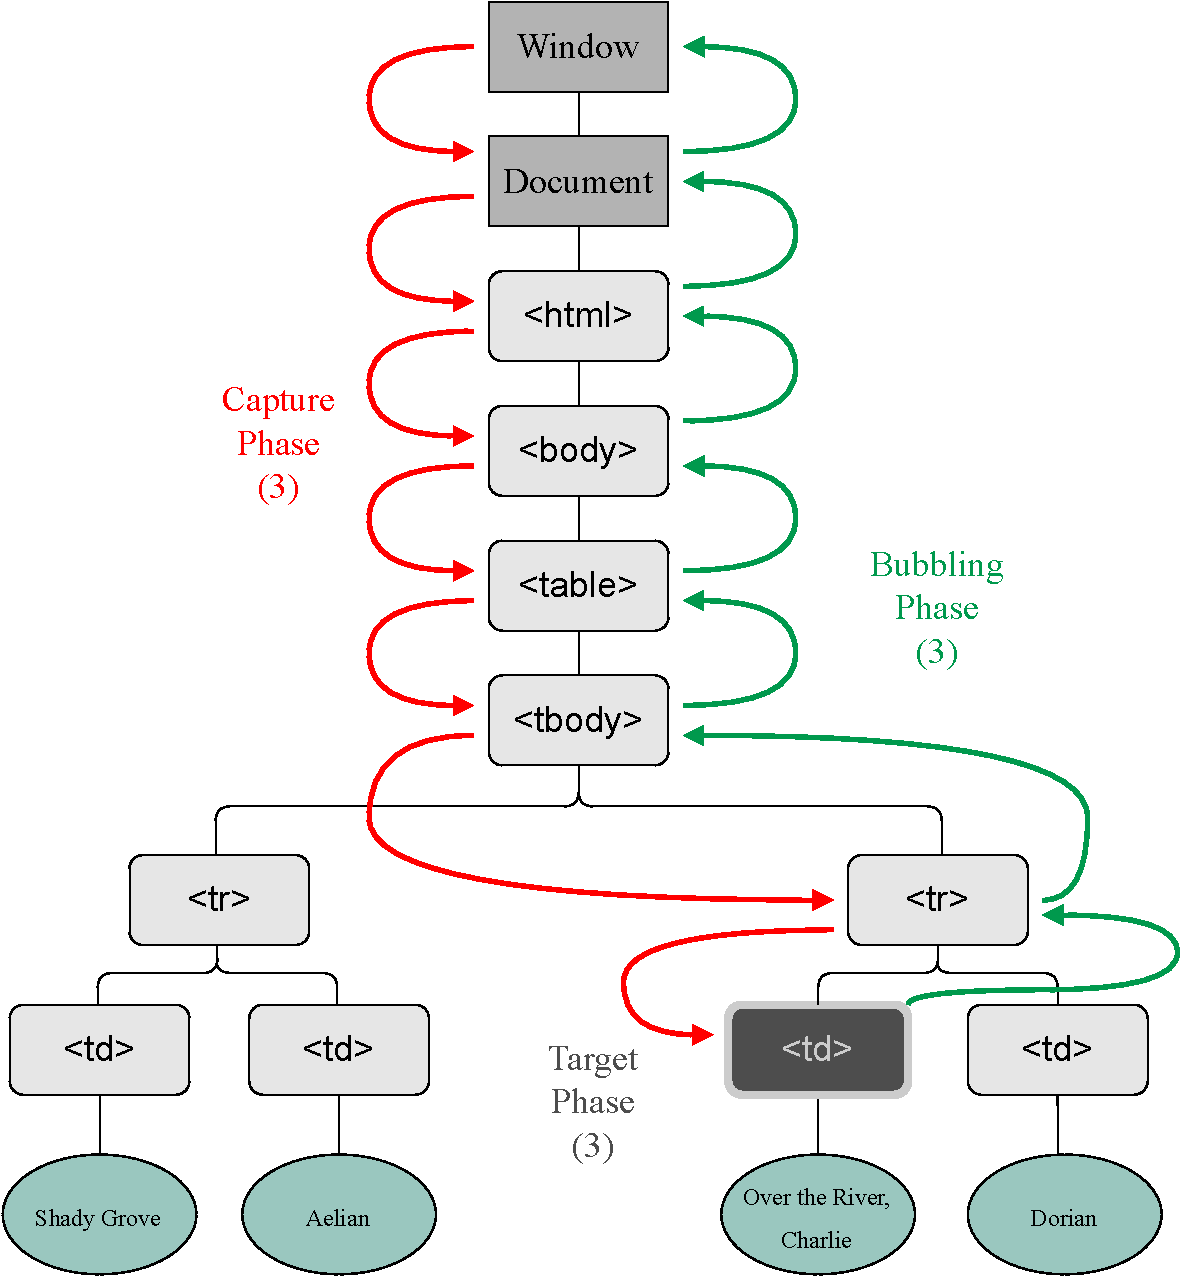
\includegraphics[width=0.65\textwidth]{Chapter2/event_bubbling/event_bubbling.pdf}
	\caption[JavaScript event propagation]
	{\textit{JavaScript event propagation}}\label{fig:ch2_event_bubbling}
\end{figure}

\Cref{fig:ch2_event_bubbling} illustrates the example of an event propagation of a child element that executes a DOM event when clicked on. Event propagation consists of three phases:

\begin{itemize}
	\item \textit{Capturing phase:} The event propagates downward to the target element with which the user interacts.
	\item \textit{Target phase:} The event reaches the targeted element to execute the DOM event.
	\item \textit{Bubbling phase:} The event bubbles up from the target element.
\end{itemize}

Capturing the targeted element may be difficult because some web pages may have more complex HTML, which can cause event propagation to fail to obtain the correct element information that the user interacts with. In such cases, obtaining the target element by identifying the last known element the user hovered over on the user interface is more accurate since another DOM event may have started during the initial element's event.\par \Cref{fig:ch3_element_event_capturing} illustrates the flow diagram to capture the element with which the user interacted for the user-based activity log. This code segment will be initiated during the \texttt{beforeSend} operation of the \textit{AJAX request} to filter HTML elements by predefined allowed elements. Filtering the element tag names ensures that unwanted, more complex, essential elements not expected to be the event's initiator will be excluded. 

\begin{figure}[!htb]
	\centering % cent the figure
	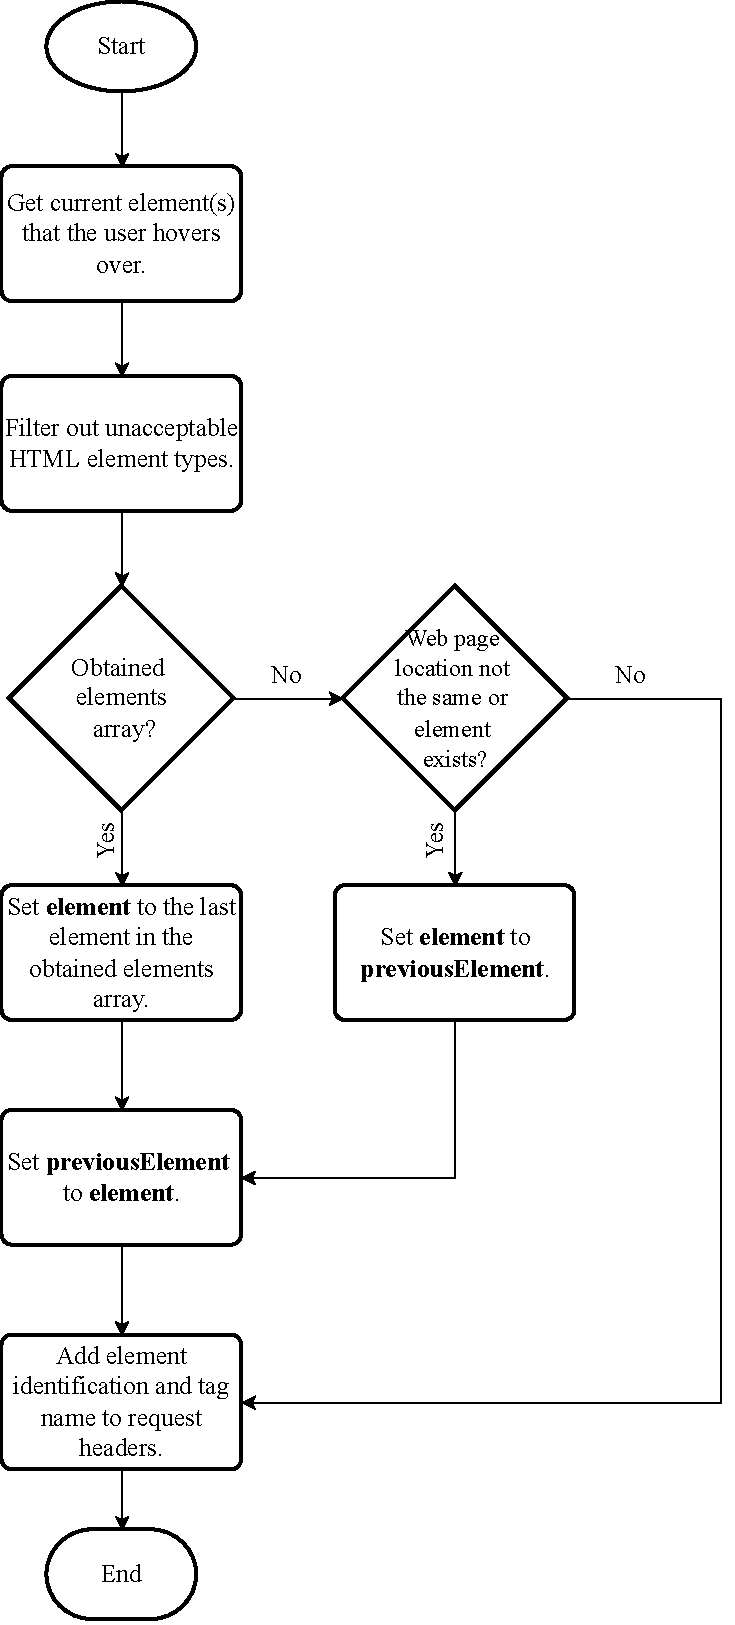
\includegraphics[width=0.55\textwidth]{Chapter2/element_capturing/element_capturing.pdf}
	\caption[HTML element capturing flow diagram]
	{\textit{HTML element capturing flow diagram}}\label{fig:ch3_element_event_capturing}
\end{figure}

If the web location has already changed or no element exists, the page's contents may have changed during the event propagation. Therefore, the last known component that the user hovered over must be used because it is most likely the element that the user interacted with. This approach ensures that a component has always been detected and synchronised with the request header in most UI changes.

\subsection{Logging points}
Table \ref{tbl:ch2_loggingPointRequirement} outlines the functional requirements for logging points in the software system. It is crucial to maintain consistency when capturing logs. Placing the captured logs globally for all HTTP requests will ensure consistency. Filters can be used during the test system, as it is an \texttt{ ASP.NET Core Web SDK}. Filters can be initialised during the software system startup phase.\par For other web-based systems, the central point where \textit{HTTP requests} are processed should be used to place single or multiple logging points. In other cases, adding it for smaller groups of subsystems is also viable if the logs can be consistently captured when requests come through. \par The filter of the test system is the primary component of the logging mechanism. Log attributes and metadata can be captured log attributes and metadata on the client side using server-side parsing, as shown in Figure \ref{fig:ch2_loggingParse}. \par \Cref{sec:ch3_implementationLogAtrributes} discussed that some of the logs may contain sensitive data that should not be logged, especially the metadata request parameters. Adding a flag to indicate that specific subsystem requests must be ignored for event logging should be included. \par This may exclude specific parameters from being saved into the database. It is an attribute added to specific controllers to ignore the event logs obtained and terminate the logging process. \par The logging process in Figure \ref{fig:ch3_loggingProcess} is placed on the client-side filter, which runs before the rest of the request is handled. It is essential to check whether the request has an action parameter to ensure that the function being executed is called by the request and not by the internal system. \par If the request has a report action parameter, the user activity should be set to either \texttt{Activity1} or \texttt{Activity2}. The rest of the request parameters should be obtained and formatted as a \texttt{JSON} string to be stored in the database.

\clearpage

\begin{figure}[!htb]
	\centering % cent the figure
	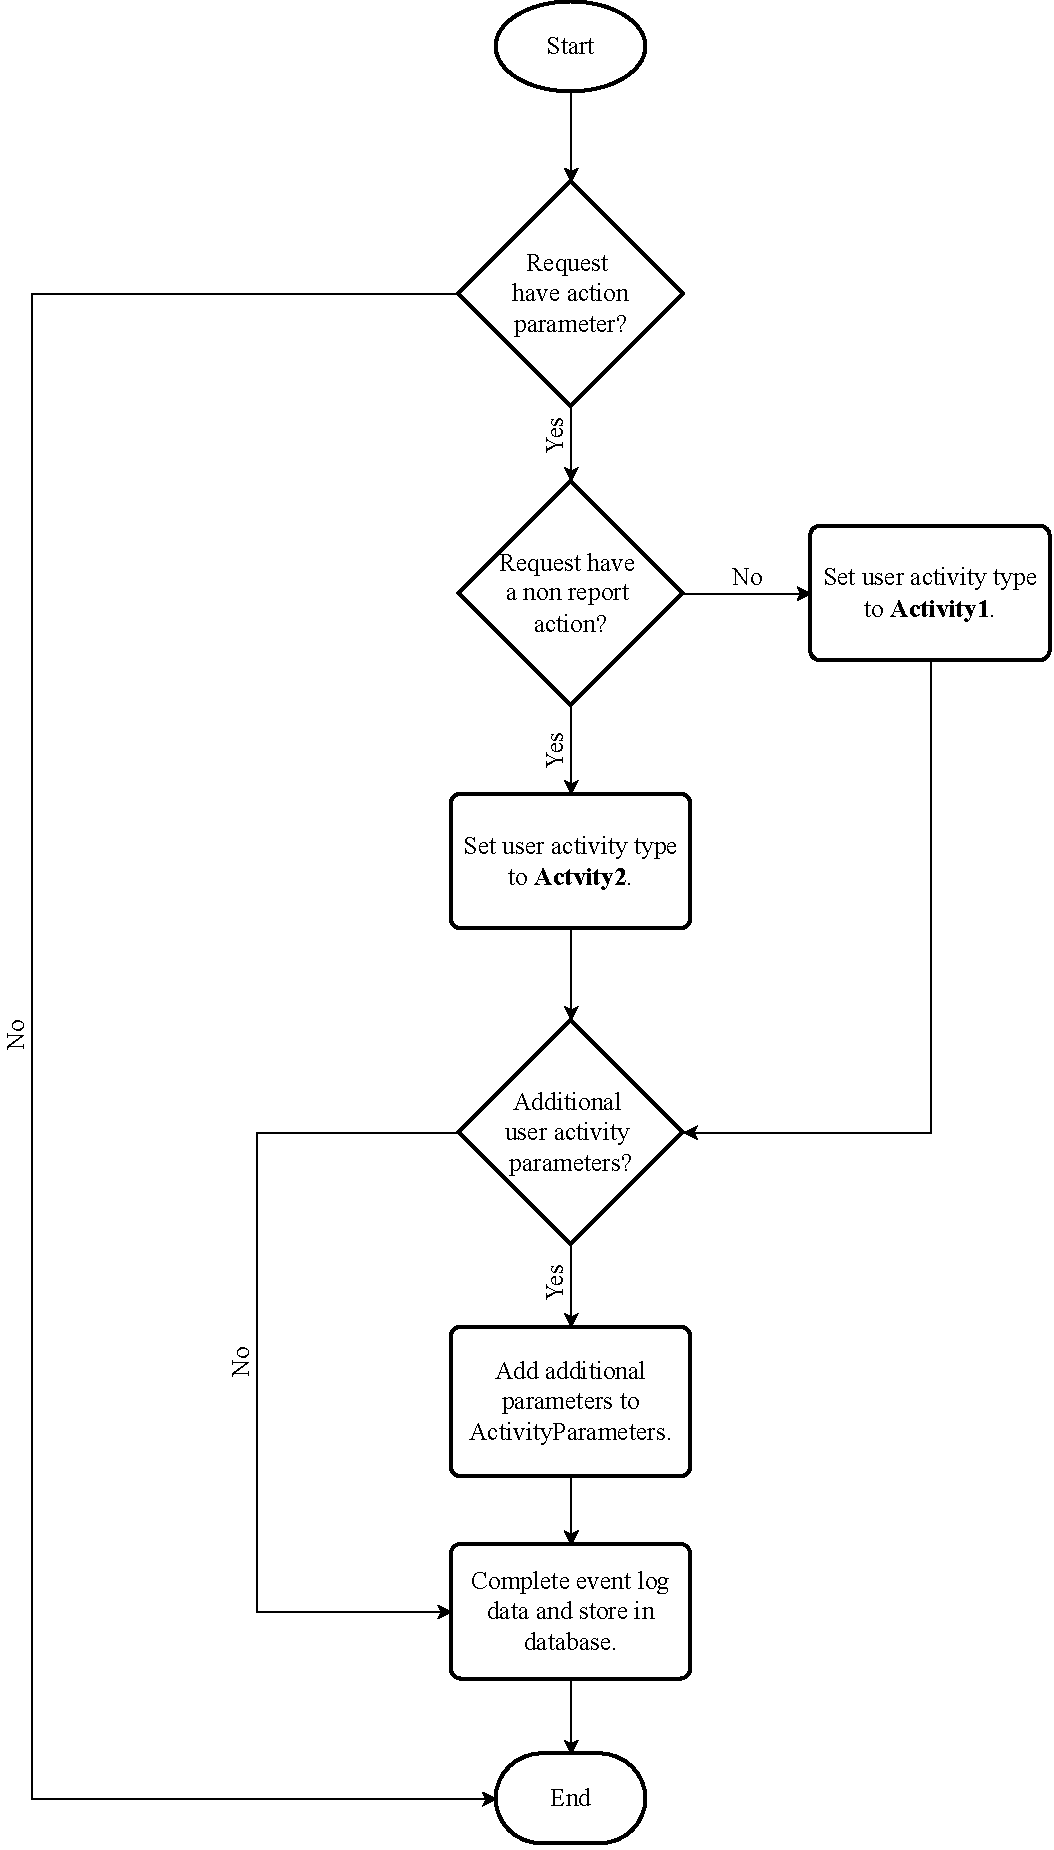
\includegraphics[width=0.8\textwidth]{Chapter2/DetailView_Flow/DetailView_Flow.pdf}
	\caption[Logging point operation for test system]
	{\textit{Logging point operation for test system}}\label{fig:ch3_loggingProcess}
\end{figure}

\clearpage

\subsection{Log analysis}\label{sec:ch3_implementationLogAnalysis}
In \Cref{sec:ch2_logAnalysisTools,sec:ch2_utilisationImprovements}, the functional requirements for log analysis are defined. For the implementation of log analysis, a custom log analysis tool is created to:

\begin{itemize}
	\item Visually present user-based event logs through the log analysis tool as outlined in \Cref{tbl:ch2_logAnalysisToolFR}.
	\item Filter user-based event logs using different criteria described in \Cref{tbl:ch2_utilisationCategories}.
	\item Analyse logs for maintenance prioritisation as shown in \Cref{tbl:ch2_maintenancePriortising}.
\end{itemize}

\section{Verification}\label{sec:ch3_Verification}
The log analysis tool will be used to verify the implementation of the logging mechanism on the test system. The log analysis tool is created in a \texttt{.NET Framework} software environment and uses a \texttt{MySQL} database to store log events.

\subsection{Log attributes}
A sample of the captured log attributes of \Cref{tbl:ch3_Log_Attributes} is shown in \Cref{fig:ch3_UAT_menu}.

\begin{figure}[!htb]
	\centering % cent the figure
	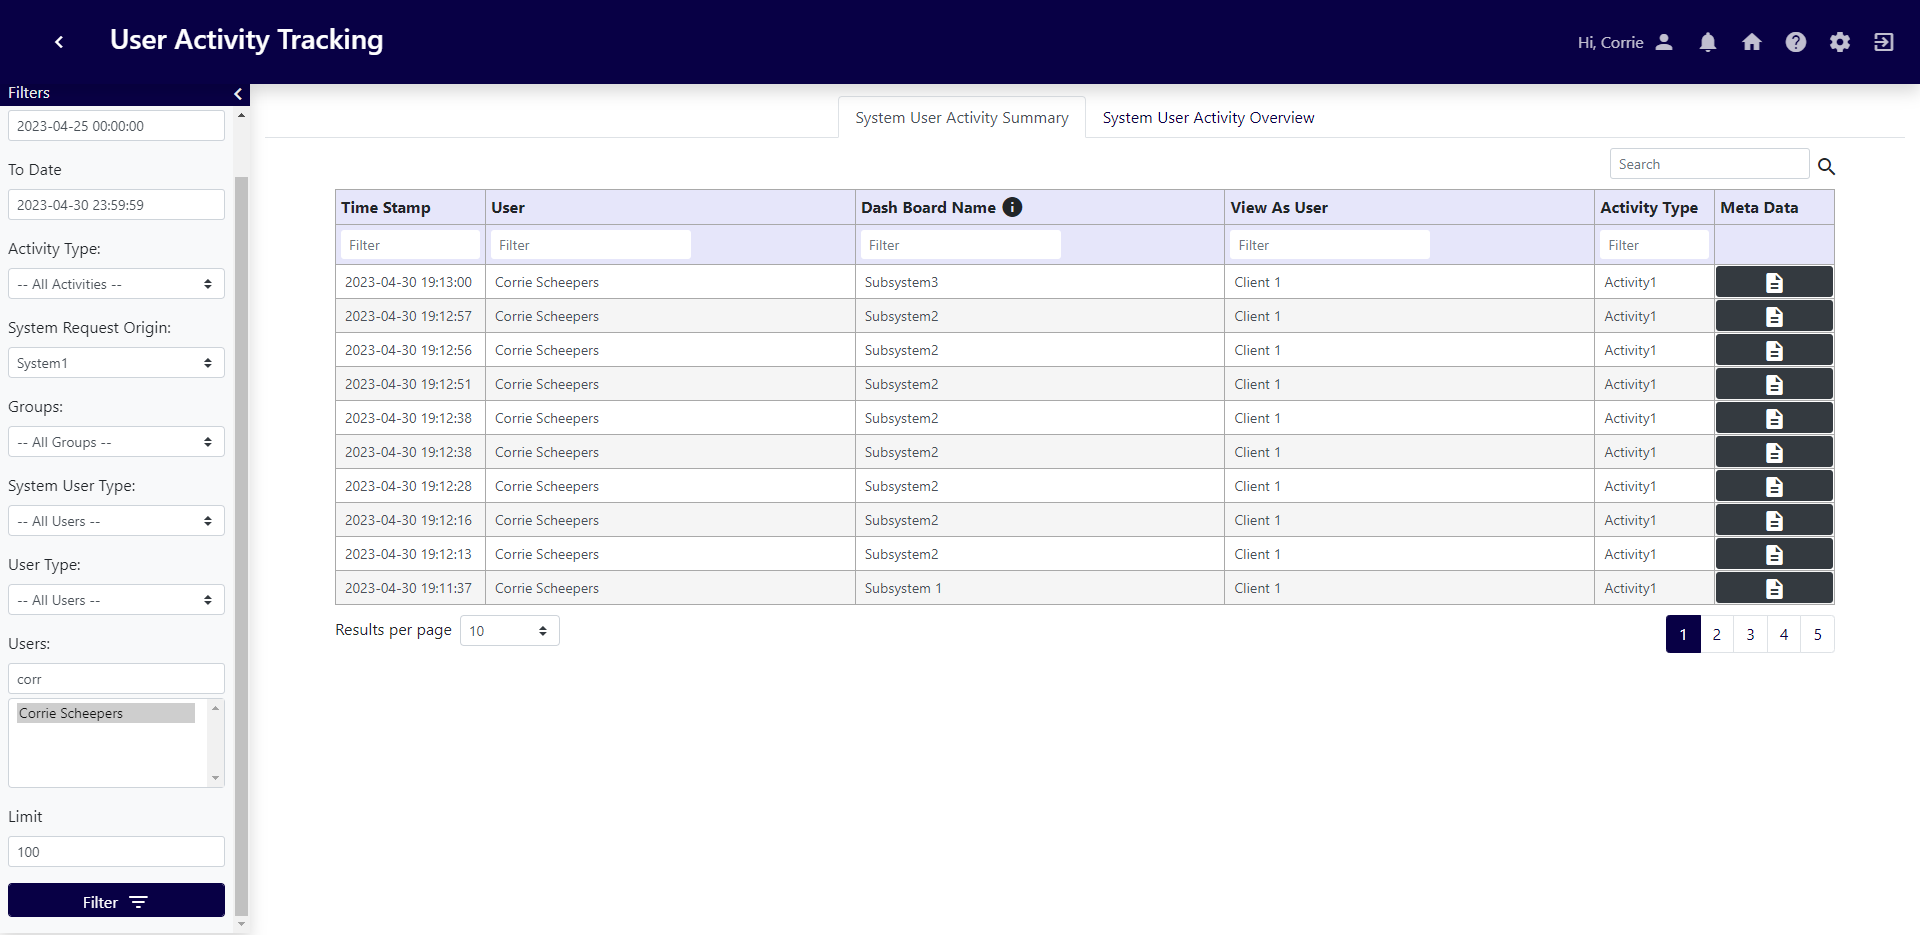
\includegraphics[width=0.99\linewidth]{img/ch3/analysis/UAT_menu.png}
	\caption[Interactive user activity viewer]
	{\textit{Interactive user activity viewer}}\label{fig:ch3_UAT_menu}
\end{figure}

\Cref{fig:ch3_UAT_menu} illustrates that the required log attributes defined in \Cref{tbl:ch3_Log_Attributes} are being tracked for the test systems. The user interface created to display the logs is designed to be more understandable to users who analyse the logs. The metadata is displayed in a \texttt{JSON} format as seen in \Cref{fig:ch3_JSON_Test_Result}.

\clearpage

\begin{figure}[!htb]
	\centering % cent the figure
	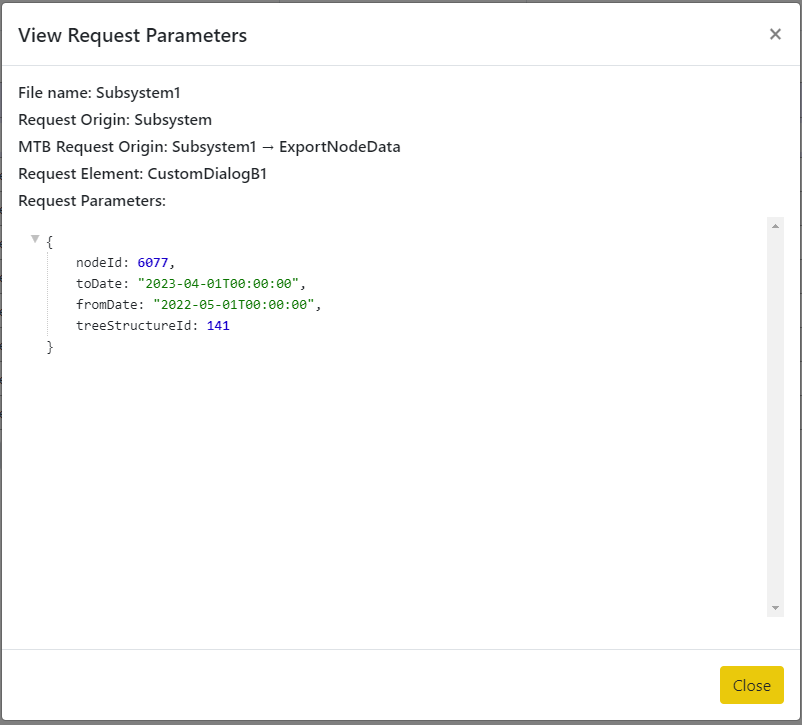
\includegraphics[width=0.6\linewidth]{img/ch3/analysis/UAT_request_params.png}
	\caption[JSON test request parameter data]
	{\textit{JSON test request parameter data}}\label{fig:ch3_JSON_Test_Result}
\end{figure}

\Cref{fig:ch3_JSON_Test_Result} includes additional parameters described in \Cref{fig:ch3_MetadataJson}. \texttt{RequestElementID} is obtained using the element capture method described in \Cref{fig:ch3_element_event_capturing}, while the other metadata parameters are captured using the built-in methods available in \texttt{C\#}.

\subsection{Log analysis}
The log analysis of the logs obtained in \Cref{fig:ch3_UAT_menu} is done in the same interactive dashboard. \Cref{fig:ch3_UAT_menuAnalysis} compares the logs obtained for the subsystems.

\begin{figure}[!htb]
	\centering % cent the figure
	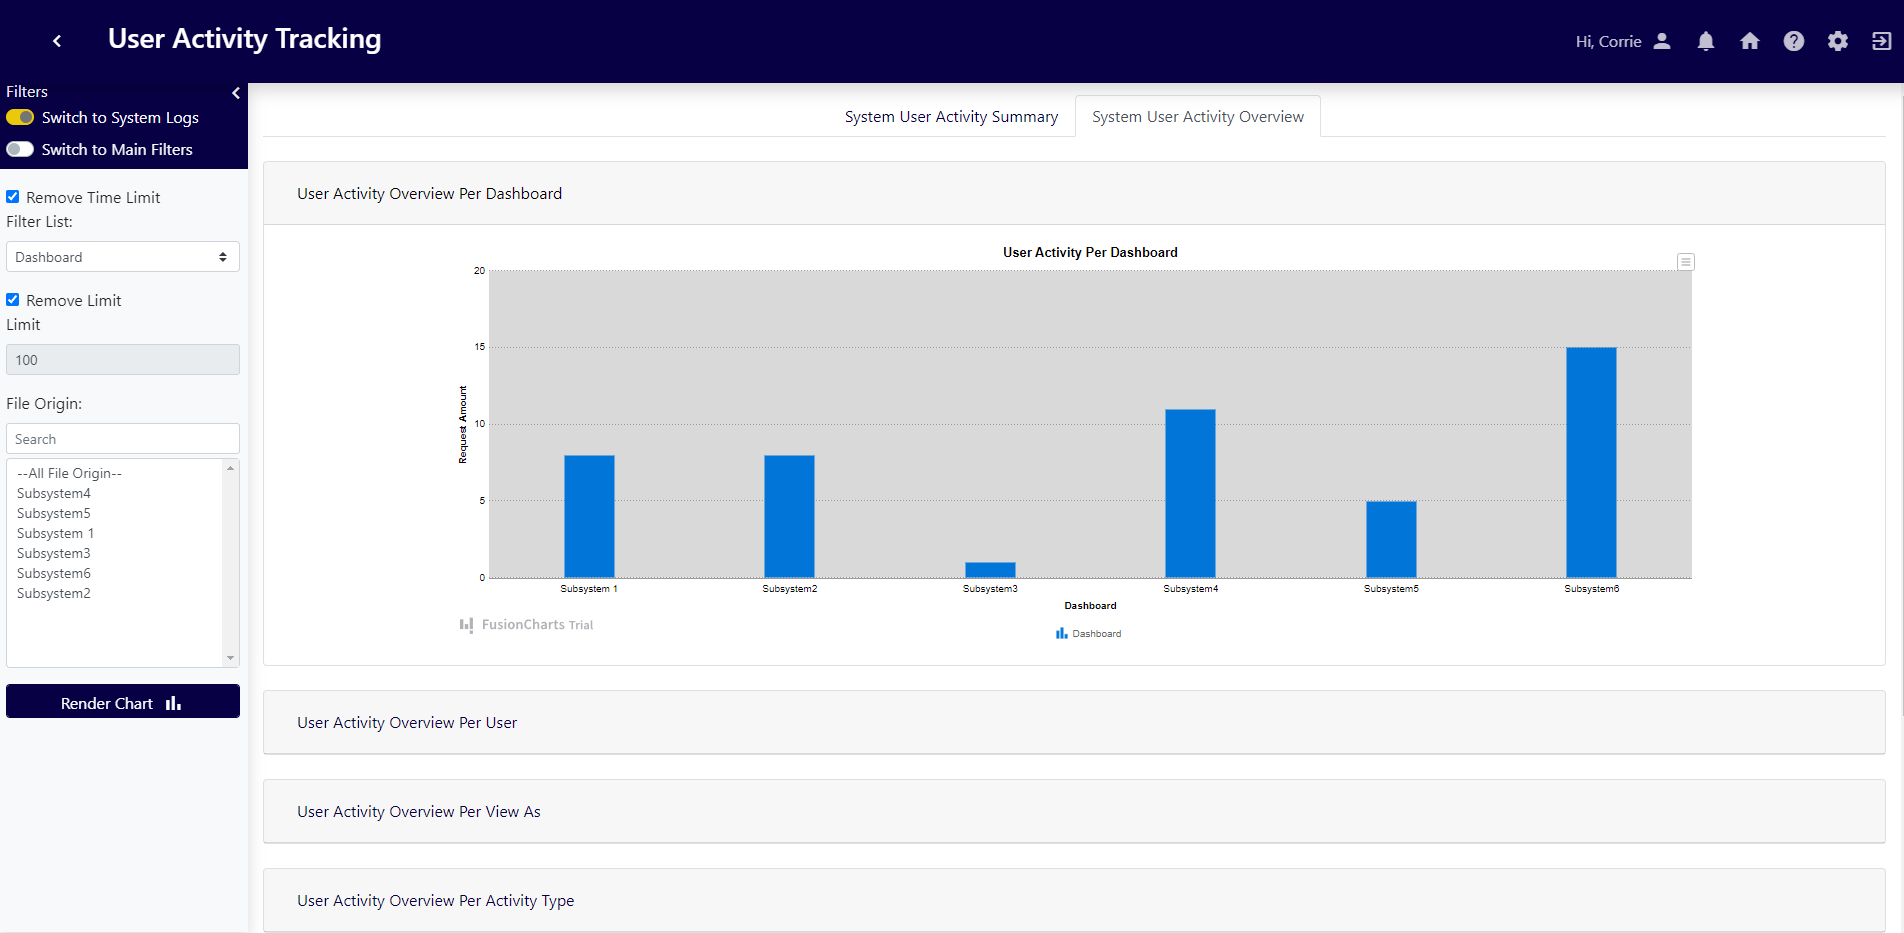
\includegraphics[width=0.99\linewidth]{img/ch3/analysis/UAT_menu_analysis.png}
	\caption[Interactive user activity viewer]
	{\textit{Interactive user activity viewer}}\label{fig:ch3_UAT_menuAnalysis}
\end{figure}

\clearpage

The log analysis, as seen in \Cref{fig:ch3_UAT_menuAnalysis}, illustrates the subsystems' total recorded user activity logs that are compared. Depending on the required logging attributes, different categorical comparisons can be made from the obtained user-based event logs. \par By comparing the categories described in \Cref{tbl:ch2_utilisationCategories}, different categories can be compared, as shown in \Cref{fig:ch3_UAT_menuAnalysis}. 

\begin{figure}[!htb]
	\centering % cent the figure
	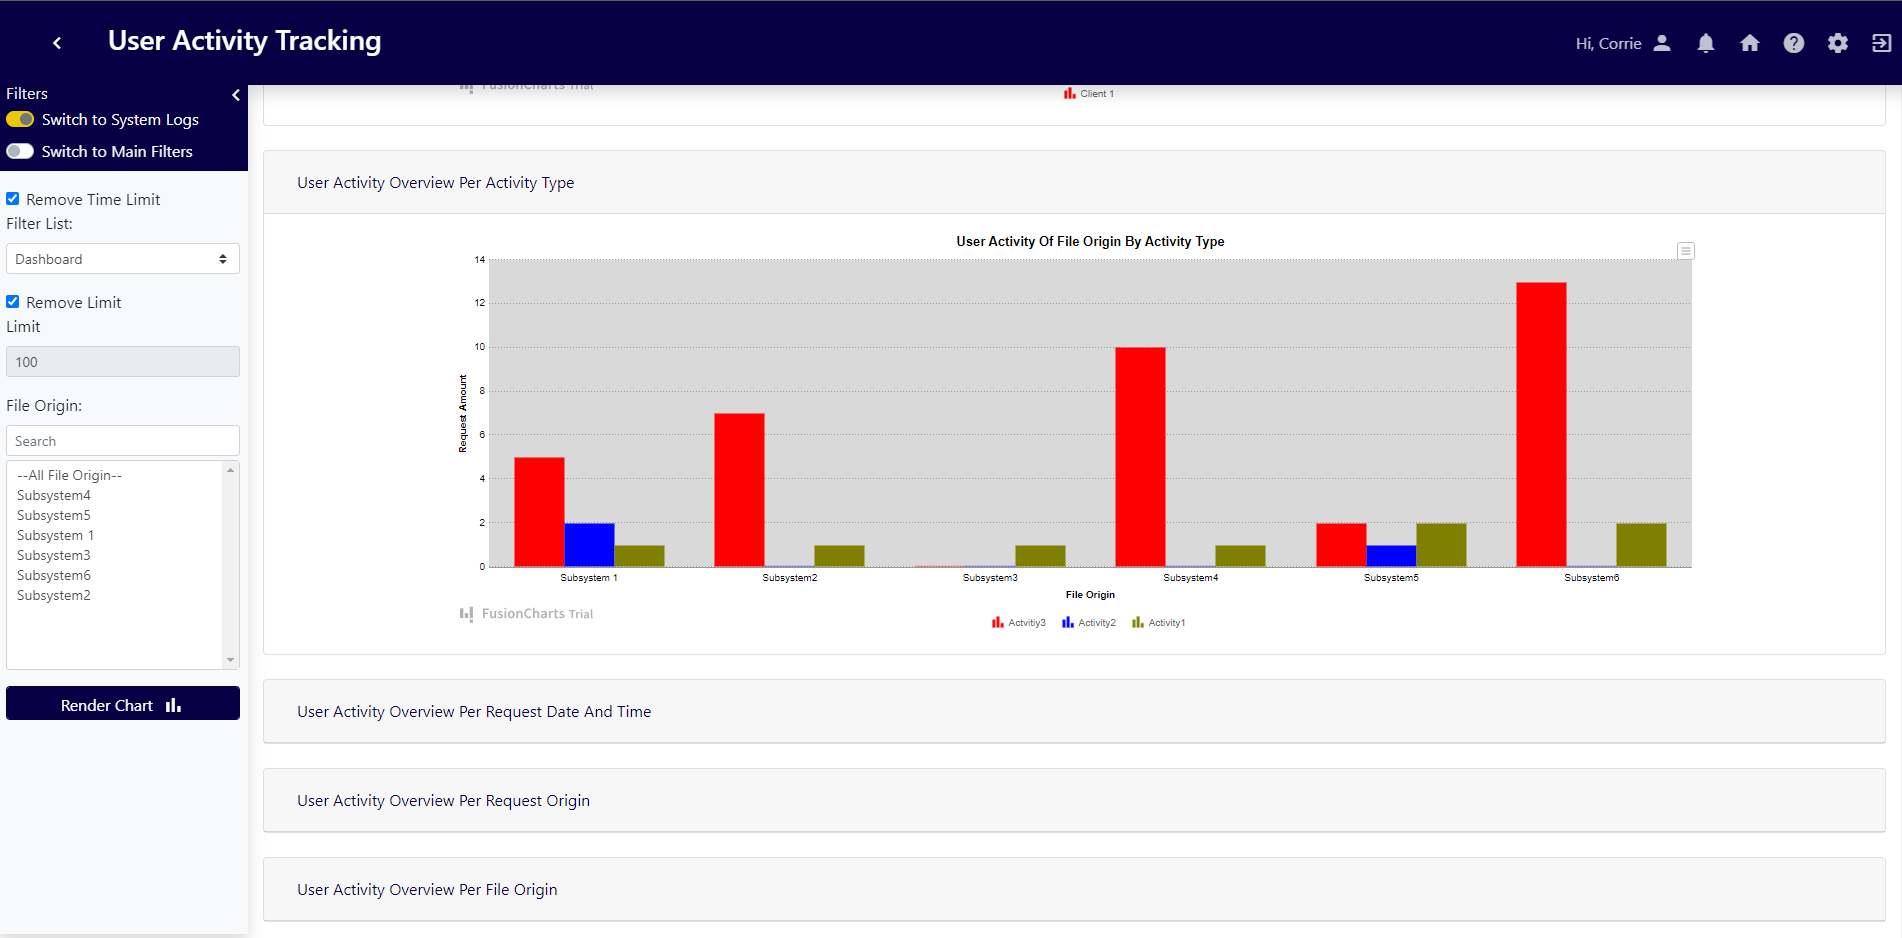
\includegraphics[width=0.99\linewidth]{img/ch3/analysis/UAT_menu_activities.png}
	\caption[Interactive user activity log analysis]
	{\textit{Interactive user activity log analysis}}\label{fig:ch3_UAT_menuActivities}
\end{figure}

\Cref{fig:ch3_UAT_menuActivities} compares user activity types. For these subsystems, \texttt{Activity3}, which is the \texttt{General} user activity type, is the most recorded user activity type. This type of activity is expected to be the most prominent for this test system. 

\clearpage

\subsubsection{Log quality}
Using the functional requirements for the log quality (\ref{fr:logQuality}), the log quality of the test system is evaluated in \Cref{tbl:ch3_testLoggingQuality}.

\begin{xltabular}{\textwidth}{clcX}
	\caption[Logging quality assessment of the test system]{\textit{Logging quality assessment of the test system}}\label{tbl:ch3_testLoggingQuality}\\
	\toprule
	\thead{Req. ID} & \thead{Description} & \thead{Achieved} & \thead{Comments} \\
	\midrule
	\endfirsthead

	\caption[]{\continueCaption} \\
	\toprule
	\thead{Req. ID} & \thead{Description} & \thead{Achieved} & \thead{Comments} \\
	\midrule
	\endhead

	\midrule
	\multicolumn{4}{r}{\continueText} \\ 
	\endfoot
	\endlastfoot

	\rowcolor{lightgray}
	\ref{fr:ur1} & Log availability & \cmark & \RaggedRight In the implementation of a logging mechanism for the test system, the log points were:
		\begin{itemize}
			\item \textit{Locally complete} since all the log attributes were available during the capturing phase of the event log.
			\item \textit{Globally complete} because defined user activity types were captured for the test system. The logging points captured the expected logs as defined in \Cref{fig:ch3_loggingProcess}.
		\end{itemize} \\
	\ref{fr:ur2} & Log completeness & \cmark & All required log attributes were obtained during the log capture process of the log point. No post-logging corrections were needed to fix any of the log attributes or to fill in missing log attributes. \\
	\rowcolor{lightgray}
	\ref{fr:ur3} & Log extraction & \cmark & As previously stated all logs were complete. Any additional information extracted from the database is to make the obtained more readable for humans by using the foreign key references to other tables as illustrated in \Cref{fig:ch2_erdOfEventLogs}. \\
	\bottomrule
\end{xltabular}

\Cref{tbl:ch3_testLoggingQuality} discussed the log quality of the test system's user-based event logs that is on an acceptable level. Log analysis should be more accurate with the concurrently obtained logs captured by the logging mechanism.

\subsection{Maintenance prioritisation}
For the test system, maintenance prioritisation recommendations can be made based on \Cref{sec:ch2_utilisationImprovements}. A rating system can be used to classify the most critical software systems that need prioritisation, which can help in software maintenance efforts. \par Using \Cref{eq:ch2_maintenanceFactorSimplified} the maintenance priority factor $M_{PF}$ can be determined for a set of systems {$S_1,~S_2,~...,~S_N$} which has captured user activities per system $A_X$. The system will also have several users connected to each system $P_X$. These parameters are set for the test system as outlined in \Cref{tbl:ch3_testData}.

\begin{table}[!htb]
	\centering
	\caption[Data for validating test system]
	{\textit{Data for validating test system}}
	\label{tbl:ch3_testData}
	\begin{tabularx}{\textwidth}{XXXX}
		\toprule
		\thead{System ($S_X$)} & \thead{Users per system ($P_X$)} & \thead{Number of events ($A_X$)} & \thead{Expected priority} \\
		\midrule
		\rowcolor{lightgray}
		$S_1$ & 226 & 11 & 1 \\
		$S_2$ & 269 & 5 & 2 \\
		\rowcolor{lightgray}
		$S_3$ & 156 & 8 & 3 \\
		$S_4$ & 155 & 1 & 5 \\
		\rowcolor{lightgray}
		$S_5$ & 146 & 13 & 5 \\
		$S_6$ & 154 & 8 & 4 \\
		\bottomrule
	\end{tabularx}
\end{table}

The activities in \Cref{tbl:ch3_testData} were generated by a single user who navigated and interacted with the system, as shown in \Cref{fig:ch3_UAT_menuActivities,fig:ch3_UAT_menuAnalysis}. To compare the effect of the total number of user activities per system, we focus on $S_3$ to $S_6$, which have similar numbers of active users who can access the system.\par For the test system $S$, it is expected that $S_1$ will have the highest maintenance priority factor, given that it has:

\begin{itemize}
	\item The second highest number of users linked to it. This should increase its normalised active user factor and
	\item has the second-highest number of observed user events captured.
\end{itemize}

$S_2$ should have the second highest expected priority. It has the highest active user count and half the total user activities captured for $S_1$. $S_3$ has a much lower user count than the two previous systems. Third, this should place its maintenance priority, as its normalised user count should be similar to $S_4$ and $S_6$. \par $S_4$ has the least number of user events but approximately the same number of users linked to it. It should, therefore, have the lowest maintenance factor since it will be zero due to normalised user activity. Similarly, \par $S_5$ will also have the lowest maintenance priority seen in $S_4$ since it has the lowest number of users connected to it. This will set the normalised priority to zero. \par $S_6$ should have the fourth highest maintenance priority. It will have a similar normalised user activity count as $S_3$ but lower normalised priority than all the systems except $S_5$. \par Using \Cref{eq:ch2_priorityNormalised} to calculate the normalised priority factor for each subsystem using the number of users that have access to the system as well as; \Cref{eq:ch2_eventNormalised} to calculate the normalised activities, the results are shown in \Cref{tbl:apx_testB_Normilised}.


    \begin{xltabular}{\textwidth}{|X|X|X|X|X|X|X|}
        \caption[Test data]
        {\textit{Test data}}
        \label{tbl:apx_testB_Normilised} \\
        
        \hline
        \textbf{$S_{X}$} & \textbf{$P_X$} & \textbf{$P_N$}  & \textbf{$A_X$} & \textbf{$A_N$} & \textbf{$M_{PF}$} & \textbf{$P_{R}$} \\
        \hline
        \endfirsthead

        \multicolumn{7}{c}
        {\tablename\ \thetable{} -- continued from previous page} \\
        \hline
        \textbf{$S_{X}$} & \textbf{$P_X$} & \textbf{$P_N$}  & \textbf{$A_X$} & \textbf{$A_N$} & \textbf{$M_{PF}$} & \textbf{$P_{R}$} \\ 
        \endhead

        \multicolumn{7}{|r|}{{Continued on next page}} \\ \hline
        \endfoot

        \hline
        \endlastfoot
    $S_1$ & 226 & 0.6504 & 11 & 0.8333 & 0.5420 & 1 \\ \hline
 $S_2$ & 269 & 1.0000 & 5 & 0.3333 & 0.3333 & 2 \\ \hline
 $S_3$ & 156 & 0.0813 & 8 & 0.5833 & 0.0474 & 3 \\ \hline
 $S_6$ & 154 & 0.0650 & 8 & 0.5833 & 0.0379 & 4 \\ \hline
 $S_4$ & 155 & 0.0732 & 1 & 0.0000 & 0.0000 & 5 \\ \hline
 $S_5$ & 146 & 0.0000 & 13 & 1.0000 & 0.0000 & 5 \\ \hline
    \end{xltabular}
    

In \Cref{tbl:apx_testB_Normilised}, $P_N$ for $S_1$ and $S_2$ is the highest, as most users have access to them. Furthermore, $S_1$ and $S_5$ have the highest $A_N$ rating, indicating that they were the most used systems. As stated, $S_1$ is expected to require the most maintenance activities. Systems with lower maintenance activities that still have similar active users linked to them have a lower maintenance priority factor.

\clearpage

\section{Case studies}\label{sec:ch3_caseStudies}

\subsection{Case study identification}
Three case studies will be used to examine the application of this study thoroughly. All the case studies are web-based applications where users need credentials to log in and have restricted access to some parts of the system. These case studies are identified in \Cref{tbl:ch3_caseStudies}.

\begin{table}[!htb]
	\centering
	\caption[Case studies]
	{\textit{Case studies}}
	\label{tbl:ch3_caseStudies}
	\begin{tabularx}{\textwidth}{clX}
		\toprule
		\thead{Case study} & \thead{Software framework} & \thead{Description} \\
		\midrule
		\rowcolor{lightgray}
		A & \texttt{ASP.NET Core Web SDK} & \RaggedRight Energy management software system comprising internal and external client users. \\
		B & \texttt{PHP} & \RaggedRight An older energy management software system comprising internal and external client users. \\
		\rowcolor{lightgray}
		C & \texttt{ASP.NET Core Web SDK} & \RaggedRight Administrative software system used by internal company users. It consists mostly of Case Study A and B configuration tools and is only accessible to internal users. \\
		\bottomrule
	\end{tabularx}
\end{table}

The case studies in \Cref{tbl:ch3_caseStudies} were selected because they have different use cases and software framework implementations. Case Studies A and B are similar software systems but use older and newer software frameworks. Due to these differences, the logging mechanism must be implemented differently to capture user-based activities. \par For the three case studies, the following results will be obtained:

\begin{itemize}
\item Defining commonly occurring user-based activity types.
\item Defining how the logging point is implemented for the specific subsystem to obtain the user-based event logs.
\item Only user activities of the subsystems in the upper quartile recorded in October 2022 are used for each case study. See \Cref{apx:caseStudies} for the results of the remaining full case studies.
\item The normalised priority for each subsystem of the main system will be calculated using \Cref{eq:ch2_priorityNormalised} based on active users who have access to the system.
\item Normalised activities of each subsystem will be calculated using \Cref{eq:ch2_eventNormalised}.
\item The maintenance priority factor will be calculated for each subsystem using \Cref{eq:ch2_maintenanceFactorSimplified}.
\item The normalisation of the priority factor is only for users who have access to the subsystem and interact with the subsystem. All other users who do not meet this requirement will be excluded.
\end{itemize}

\subsection{Case Study A results}\label{sec:ch3_csA}
Case Study A is a software system \texttt{ASP.NET Core Web SDK}. The software system has three basic user activity types, as shown in \Cref{tbl:ch3_systemAActivityTypes}.

\begin{table}[!htb]
	\centering
	\caption[Case Study A activity types]{\textit{Case Study A activity types}}
	\label{tbl:ch3_systemAActivityTypes}
	\begin{tabularx}{\textwidth}{llX}
		\toprule
		\thead{Activity} & \thead{Functional requirement} & \thead{Description} \\
		\midrule
		\rowcolor{lightgray}
		\texttt{Dash} & \ref{fr:uatType1} & \RaggedRight This activity type detects when a user has navigated to a certain subsystem. \\ 
		\texttt{DetailView} & \ref{fr:uatType3} & \RaggedRight This general activity type is for all other activities that the user initiates that send \textit{HTTP requests} back to the server.  \\
		\rowcolor{lightgray}
		\texttt{Report} & \ref{fr:uatType3} & \RaggedRight The other main function of the system is for reporting purposes. \\ 
		\bottomrule
	\end{tabularx}
\end{table}

The logging point is placed in a central location in the software code to capture the types of user activity defined in \Cref{tbl:ch3_systemAActivityTypes}. Using the action filters available in \texttt{ ASP.NET Core}, the single logging point can be placed in the software system to capture the user-based event logs. \par Additional metadata, such as the HTML element associated with the user-based event, is also captured. Using the HTML event capture method shown in \Cref{fig:ch3_element_event_capturing}, element information is captured and stored together with the request parameters in the same format described in \Cref{fig:ch3_MetadataJson}. \Cref{fig:ch3_caseABreakdown} breaks down total user activities captured of the user activity types of \Cref{tbl:ch3_systemAActivityTypes}.

\clearpage

\begin{figure}[!htb]
	\centering % cent the figure
	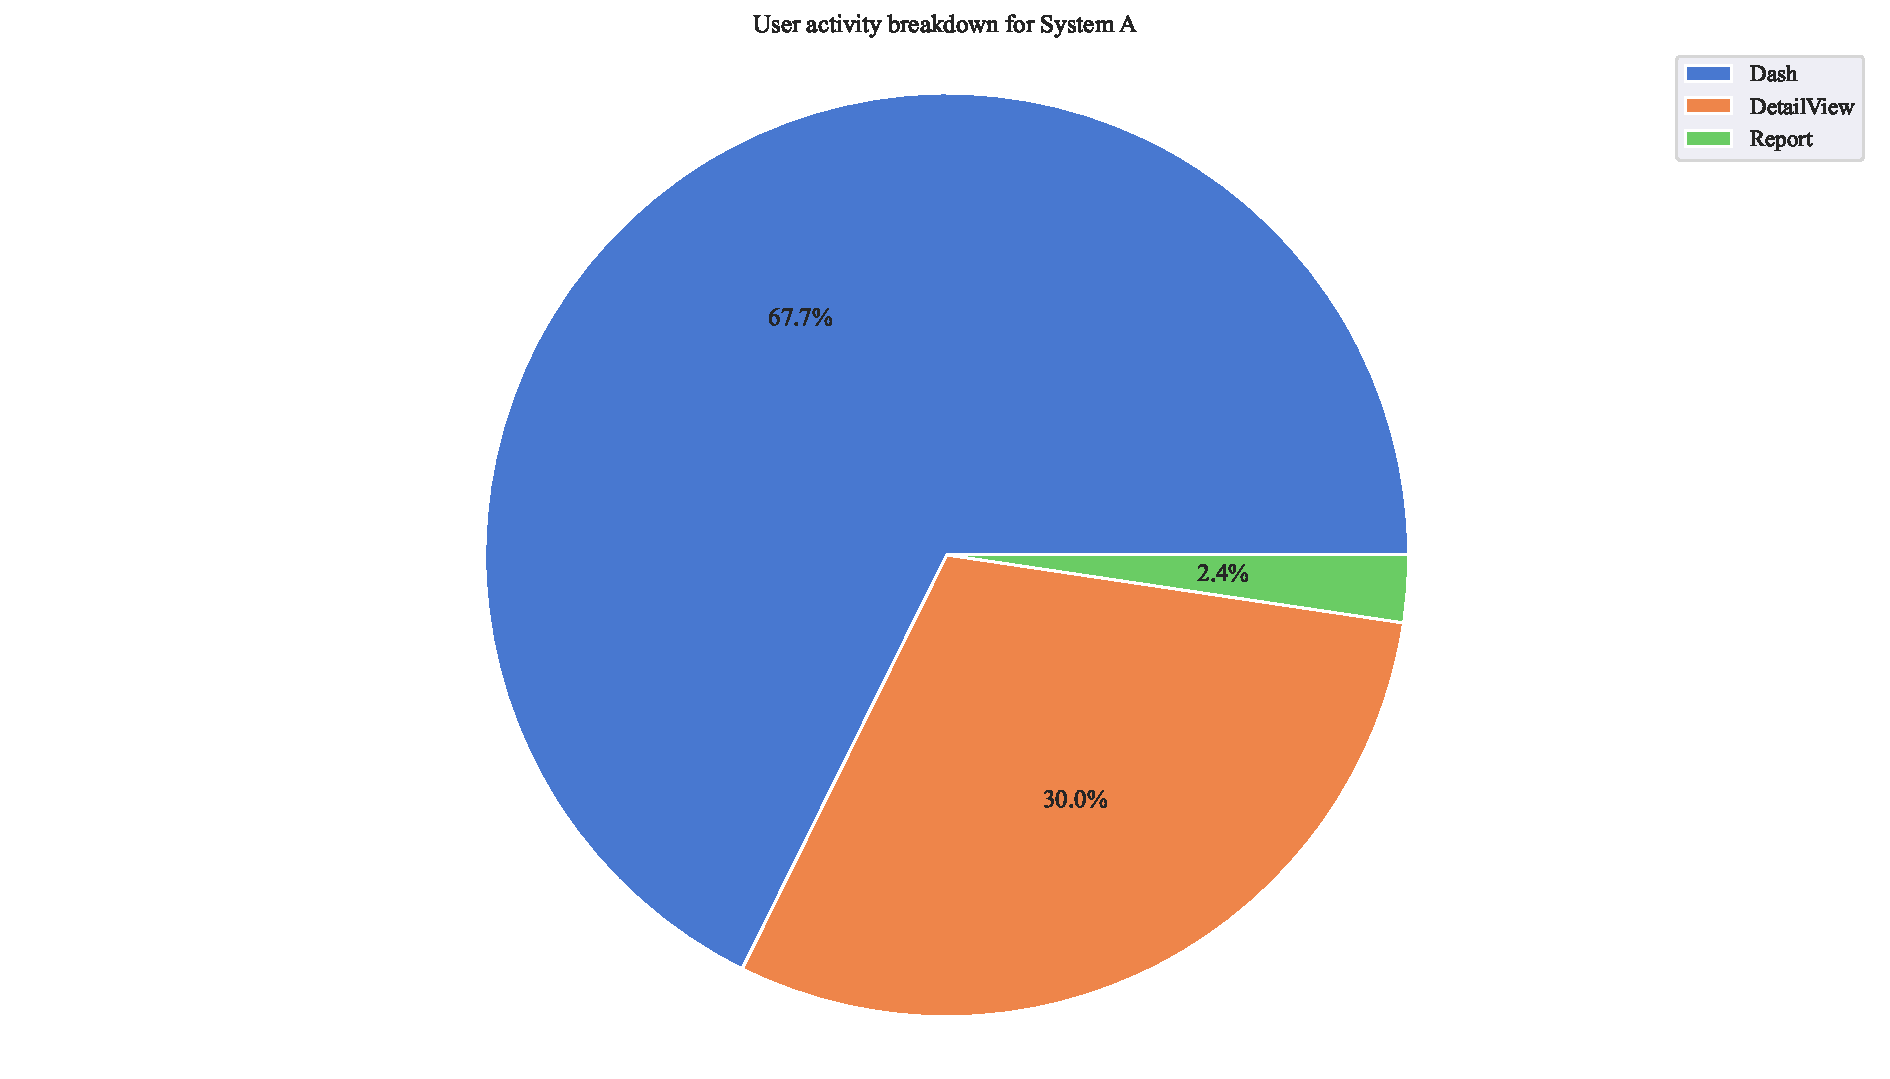
\includegraphics[width=0.95\linewidth]{img/ch3/analysis/case_A_breakdown.pdf}
	\caption[User activity types breakdown of Case Study A]
	{\textit{User activity types breakdown of Case Study A}}\label{fig:ch3_caseABreakdown}
\end{figure} 

\Cref{fig:ch3_caseABreakdown} highlights that most of the user activities for Case Study A's subsystems are the Dash user activity type. Most subsystems do not have many inputs for the user to enter data into the system. \Cref{fig:ch3_caseABreakdown} provides information back to the user that causes most of the user activities. \Cref{fig:ch3_caseAAnalysis} breaks down each subsystem's utilisation user activity.

\begin{figure}[!htb]
	\centering % cent the figure
	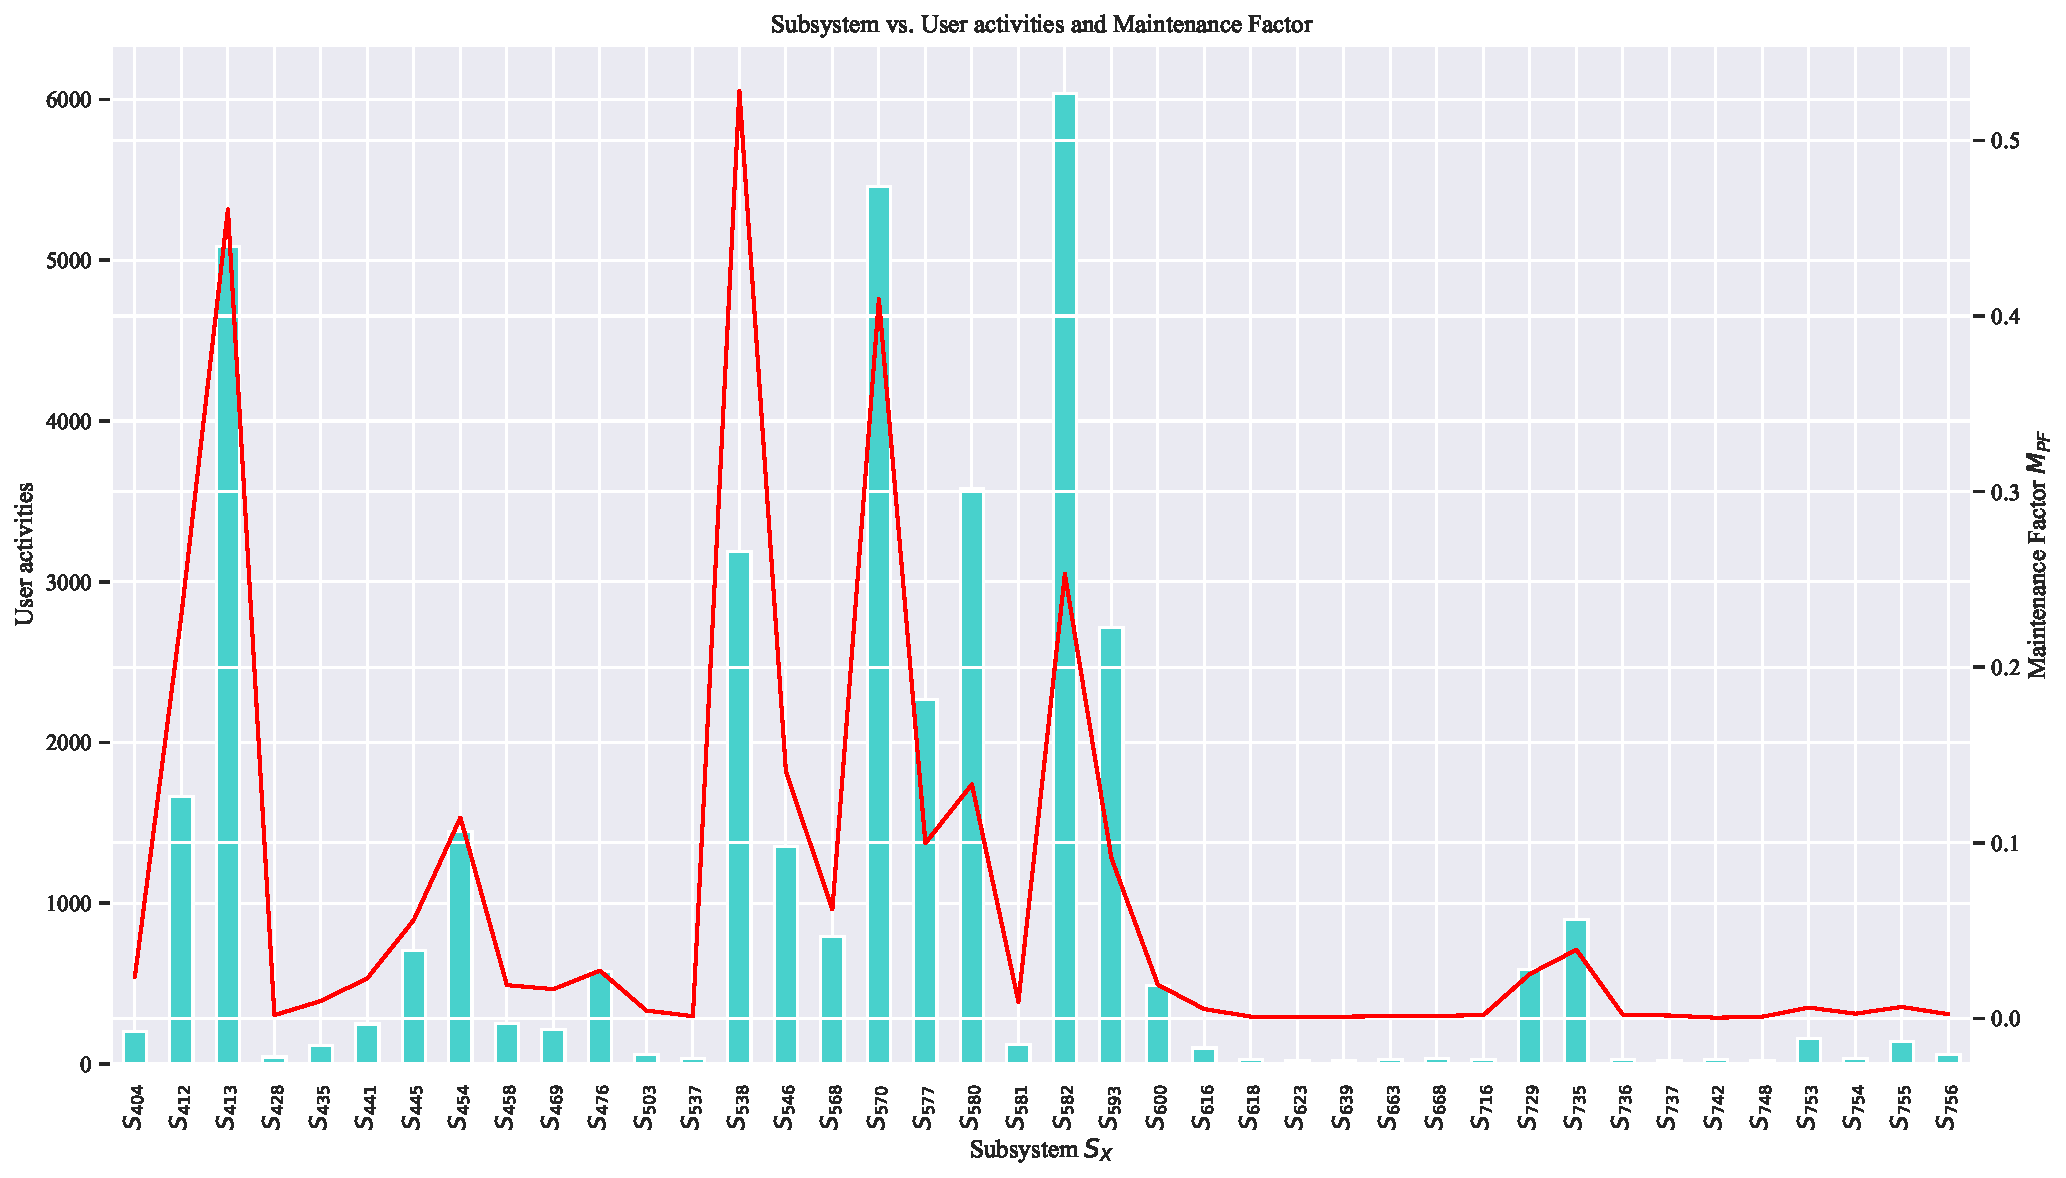
\includegraphics[width=0.95\linewidth]{img/ch3/analysis/case_A_subsystems_1.pdf}
	\caption[System utilisation breakdown of Case Study A]
	{\textit{System utilisation breakdown of Case Study A}}\label{fig:ch3_caseAAnalysis}
\end{figure}

In \Cref{fig:ch3_caseAAnalysis}, each subsystem's total utilisation is further broken down into user activity types defined in \Cref{tbl:ch3_systemAActivityTypes}. For systems such as $S_{413}$, most user activities were from actions the user performed other than accessing the subsystem, which is the DetailView user activity type. This differs from the other top five systems, with most Dash user activity types. Users only viewed the content of the web page for that subsystem. The log quality assessment for Case Study A is discussed in \Cref{tbl:ch3_caseAQuality}.

\begin{xltabular}{\textwidth}{clcX}
	\caption[Logging quality assessment of Case Study A]{\textit{Logging quality assessment of the test system}}\label{tbl:ch3_caseAQuality}\\
	\toprule
	\thead{Req. ID} & \thead{Description} & \thead{Achieved} & \thead{Comments} \\
	\midrule
	\endfirsthead

	\caption[]{\continueCaption} \\
	\toprule
	\thead{Req. ID} & \thead{Description} & \thead{Achieved} & \thead{Comments} \\
	\midrule
	\endhead

	\midrule
	\multicolumn{4}{r}{\continueText} \\ 
	\endfoot
	\endlastfoot

	\rowcolor{lightgray}
	\ref{fr:ur1} & Log availability & \cmark & \RaggedRight The log availability for Case Study A is:
		\begin{itemize}
			\item \textit{Locally complete} since all the log attributes were available during the capturing phase of the event log. 
			\item \textit{Globally complete} due to using a central logging mechanism in the main system that can capture user-based events.  
		\end{itemize} \\
	\ref{fr:ur2} & Log completeness & \cmark & This system uses the same log attribute structure described in \Cref{tbl:ch3_Log_Attributes} that is captured with the client- and server-side logging points of this case study. All the log attributes formed a complete log without additional post-logging operations to correct or fill in missing attributes. \\
	\rowcolor{lightgray}
	\ref{fr:ur3} & Log extraction & \cmark & As previously stated all the logs were \textit{locally}-and \textit{globallly} complete. This enables log extraction during log analysis. \\
	\bottomrule
\end{xltabular}

Case Study A's log quality is satisfactory for the log analysis. The three basic user activity types allow the logging points to make simple operations to classify the user-based activities. 

\clearpage

\subsubsection{Maintenance prioritisation}
The maintenance prioritisation factor for the user activities in the upper quartile of the subsystem for Case Study A is calculated in \Cref{tbl:apx_caseA}.


    \begin{xltabular}{\textwidth}{XPPPP}
        \caption[Case study A's upper quartile maintenance pefromance]
        {\textit{Case study A's upper quartile maintenance pefromance}}
        \label{tbl:apx_caseA} \\
        \toprule
         \thead{$S_{X}$} & \thead{$P_N$}  & \thead{$A_N$} & \thead{$M_{PF}$} & \thead{$P_{R}$} \\
        \midrule
        \endfirsthead

        \caption[]{\continueCaption} \\
        \toprule
        \thead{$S_{X}$} & \thead{$P_N$}  & \thead{$A_N$} & \thead{$M_{PF}$} & \thead{$P_{R}$} \\
        \midrule
        \endhead

        \midrule
        \multicolumn{5}{r}{\continueText} \\ 
        \endfoot
        \endlastfoot
    \rowcolor{lightgray} $S_{538}$ & 1.0000 & 0.5281 & 0.5281 & 1 \\ 
  $S_{413}$ & 0.5469 & 0.8423 & 0.4606 & 2 \\ 
 \rowcolor{lightgray} $S_{570}$ & 0.4531 & 0.9041 & 0.4097 & 3 \\ 
  $S_{582}$ & 0.2531 & 1.0000 & 0.2531 & 4 \\ 
 \rowcolor{lightgray} $S_{412}$ & 0.8344 & 0.2753 & 0.2297 & 5 \\ 
  $S_{546}$ & 0.6281 & 0.2240 & 0.1407 & 6 \\ 
 \rowcolor{lightgray} $S_{580}$ & 0.2250 & 0.5923 & 0.1333 & 7 \\ 
  $S_{454}$ & 0.4781 & 0.2392 & 0.1144 & 8 \\ 
 \rowcolor{lightgray} $S_{577}$ & 0.2656 & 0.3755 & 0.0997 & 9 \\ 
  $S_{593}$ & 0.2031 & 0.4496 & 0.0913 & 10 \\ 
 \rowcolor{lightgray} $S_{568}$ & 0.4719 & 0.1315 & 0.0621 & 11 \\ 
  $S_{445}$ & 0.4813 & 0.1166 & 0.0561 & 12 \\ 
 \rowcolor{lightgray} $S_{735}$ & 0.2625 & 0.1487 & 0.0390 & 13 \\ 
  $S_{476}$ & 0.2844 & 0.0956 & 0.0272 & 14 \\ 
 \rowcolor{lightgray} $S_{729}$ & 0.2594 & 0.0976 & 0.0253 & 15 \\ 
  $S_{404}$ & 0.7000 & 0.0338 & 0.0237 & 16 \\ 
 \rowcolor{lightgray} $S_{441}$ & 0.5563 & 0.0411 & 0.0229 & 17 \\ 
  $S_{600}$ & 0.2375 & 0.0808 & 0.0192 & 18 \\ 
 \rowcolor{lightgray} $S_{458}$ & 0.4500 & 0.0421 & 0.0189 & 19 \\ 
  $S_{469}$ & 0.4656 & 0.0358 & 0.0167 & 20 \\ 
 \rowcolor{lightgray} $S_{435}$ & 0.5156 & 0.0192 & 0.0099 & 21 \\ 
  $S_{581}$ & 0.4750 & 0.0200 & 0.0095 & 22 \\ 
 \rowcolor{lightgray} $S_{755}$ & 0.2812 & 0.0232 & 0.0065 & 23 \\ 
  $S_{753}$ & 0.2375 & 0.0258 & 0.0061 & 24 \\ 
 \rowcolor{lightgray} $S_{616}$ & 0.3219 & 0.0164 & 0.0053 & 25 \\ 
  $S_{503}$ & 0.4500 & 0.0099 & 0.0045 & 26 \\ 
 \rowcolor{lightgray} $S_{756}$ & 0.2375 & 0.0099 & 0.0024 & 27 \\ 
  $S_{428}$ & 0.2594 & 0.0071 & 0.0018 & 28 \\
        \bottomrule
    \end{xltabular}
    

\Cref{tbl:apx_caseA} shows the results of the implementation \Cref{eq:ch2_priorityNormalised,eq:ch2_eventNormalised,eq:ch2_maintenanceFactorSimplified} to calculate the normalised priority ($P_N$), normalised activity ($A_X$), and maintenance factor ($M_{PF}$) respectively. \Cref{tbl:apx_caseA} only contains the upper quartile subsystems of all the total subsystems of \Cref{tbl:apx_projectA_Normilised} in \Cref{tbl:apx_caseB}. The results are visually presented in \Cref{fig:ch3_caseAAnalysis} collected from \Cref{tbl:apx_caseA} with the breakdown of user activity. \par In \Cref{fig:ch3_caseAAnalysis}, subsystem $S_{582}$ had the most user-generated events, with an average of $72.75$ user-generated events per user. The lower $P_N$ reduced its maintenance priority factor to the highest $4_{th}$ for all subsystems. The subsystem $S_{538}$ had the $5^{th}$ highest number of recorded user-based activities and the most users with access to the subsystem. The higher $P_N$ had a greater impact on its maintenance performance factor. 

\clearpage

\subsection{Case Study B results}\label{sec:ch3_csB}
Case Study B is implemented on an older system than Case Studies A and C and is primarily created in \texttt{PHP}. This system has the same type of user activities as Case Study A's \Cref{tbl:ch3_systemAActivityTypes}. This system used multiple logging points to capture the types of users of \Cref{tbl:ch3_systemAActivityTypes}. \par The purpose of the use of numerous logging points was to:

\begin{itemize}
	\item Ensure each subsystem's user activities could be captured since there was no central point in the software architecture to capture the request. 
	\item The system comprised groups of smaller software systems where the logging points could be added.
	\item Some adjustments had to be made to the logging points to ensure that the quality of the log was maintained when it was captured. 
	\item Consistency was also important, so each logging has several minor differences added to ensure it can consistently capture certain user-based events.
\end{itemize}

The logging points do not track any of the elements that the user interacted with in the system. Only a portion of the request parameters are tracked for user-based activities. The metadata will contain only the \texttt{RequestParameters} used in \Cref{fig:ch3_MetadataJson}. The breakdown of user activity types for this case study is shown in \Cref{fig:ch3_caseBBreakdown}.

\begin{figure}[!htb]
	\centering % cent the figure
	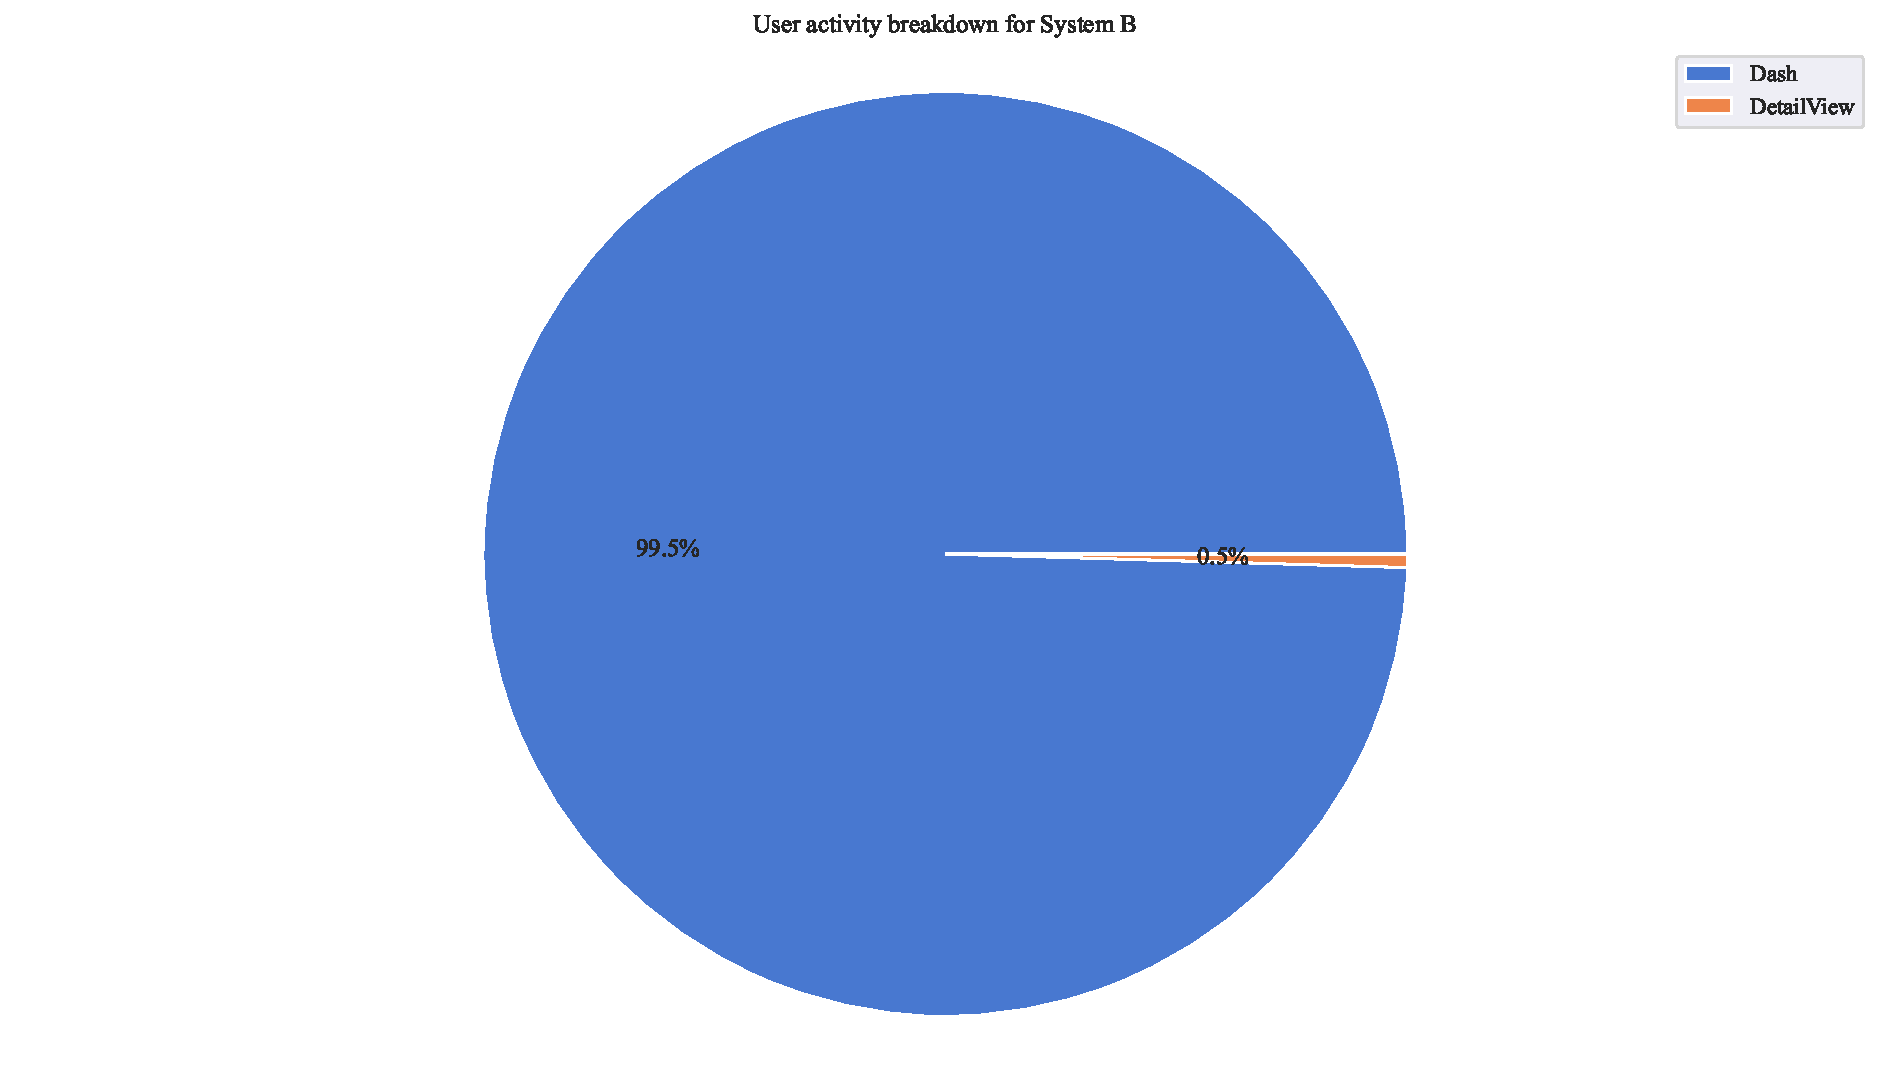
\includegraphics[width=0.95\linewidth]{img/ch3/analysis/case_B_breakdown.pdf}
	\caption[User activity types breakdown of Case Study B]
	{\textit{User activity types breakdown of Case Study B}}\label{fig:ch3_caseBBreakdown}
\end{figure}

In \Cref{fig:ch3_caseBBreakdown}, the \texttt{Dash} user activity type is approximately $99.5\%$ of all user activities recorded. Case Study B has fewer subsystems that require the user to interact with the web page to accumulate data. The system mainly comprises web pages that display data only for the user. There were no \texttt{Report} user activity types as the users did not create reports to export from these subsystems. \Cref{fig:ch3_caseBAnalysis} breaks down each subsystem's utilisation user activity.

\begin{figure}[!htb]
	\centering % cent the figure
	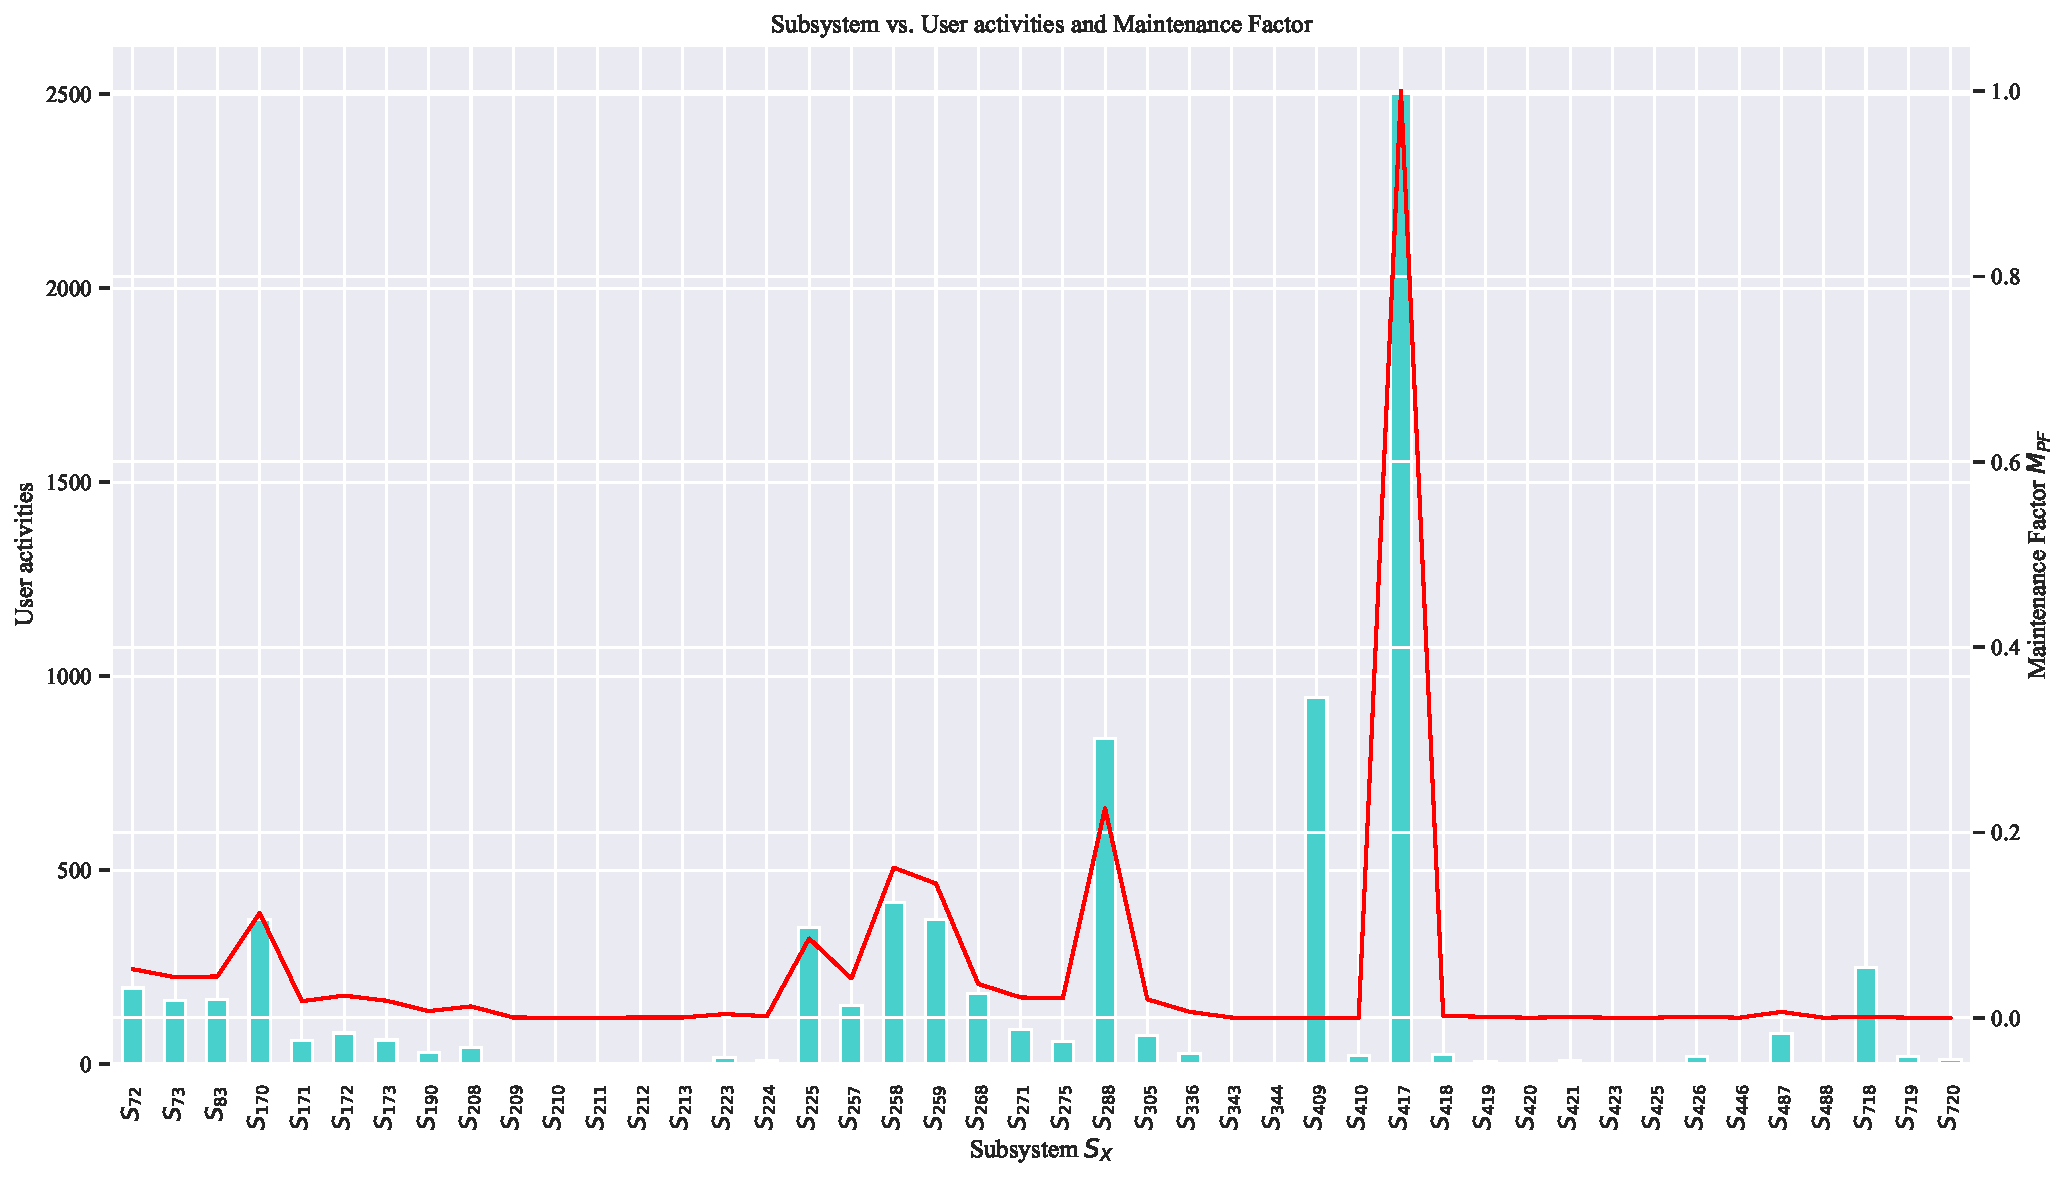
\includegraphics[width=0.95\linewidth]{img/ch3/analysis/case_B_subsystems_1.pdf}
	\caption[System utilisation breakdown of Case Study B]
	{\textit{System utilisation breakdown of Case Study B}}\label{fig:ch3_caseBAnalysis}
\end{figure} 

In \Cref{fig:ch3_caseBAnalysis}, all the subsystems have the majority \texttt{Dash} user activity type. Approximately $99.5\%$ of the user activities are \texttt{Dash} user activity because the older system made in \texttt{PHP} is only used for monitoring energy systems. The subsystems have simple inputs, such as date pickers and category pickers. These input types only refresh the page, which causes more \texttt{Dash} activities to load new data for the user. \par $S_{417}$ has the most user activities, approximately $2.5$ times higher than the second system, $S_{409}$, and has the most active users in this system. The log quality assessment for Case Study B is discussed in \Cref{tbl:ch3_caseBQuality}.

\begin{xltabular}{\textwidth}{clcX}
	\caption[Logging quality assessment of Case Study B]{\textit{Logging quality assessment of Case Study B}}\label{tbl:ch3_caseBQuality}\\
	\toprule
	\thead{Req. ID} & \thead{Description} & \thead{Achieved} & \thead{Comments} \\
	\midrule
	\endfirsthead

	\caption[]{\continueCaption} \\
	\toprule
	\thead{Req. ID} & \thead{Description} & \thead{Achieved} & \thead{Comments} \\
	\midrule
	\endhead

	\midrule
	\multicolumn{4}{r}{\continueText} \\
	\endfoot
	\endlastfoot

	\rowcolor{lightgray}
	\ref{fr:ur1} & Log availability & Mostly & \RaggedRight The log availability for Case Study B is:
		\begin{itemize}
			\item Mostly \textit{locally complete} since all the log attributes were available during the capturing phase of the event log. Each log point had its method of obtaining the same log attributes.
			\item Mostly \textit{globally complete} due to multiple logging mechanisms. They may have differences in their ability to identify a user-based event and capture the necessary log attributes to complete the log. 
		\end{itemize} \\
	\ref{fr:ur2} & Log completeness & Mostly & The use of multiple logging points will yield different results in the same main software system. Some post-logging operations may be needed to fix and exclude some event logs. \\
	\rowcolor{lightgray}
	\ref{fr:ur3} & Log extraction & \cmark & Although the availability and completeness of the event logs are generally achieved, the log extraction process is still possible.   \\
	\bottomrule
\end{xltabular}

\Cref{tbl:ch3_caseBQuality} emphasises the issues of using multiple logging points with different operations to obtain user-based events. Case Study B used post-logging operations in the log analysis tool to exclude some unfixable logs, make applicable corrections, and fill in missing log attributes based on other log attributes.

\clearpage

\subsubsection{Maintenance prioritisation}
The maintenance prioritisation factor for the user activities in the upper quartile of the subsystem for Case Study B is calculated in \Cref{tbl:apx_caseB}.


    \begin{xltabular}{\textwidth}{XXXXX}
        \caption[Case study B's upper quartile maintenance pefromance]
        {\textit{Case study B's upper quartile maintenance pefromance}}
        \label{tbl:apx_caseB} \\
        \toprule
         \thead{$S_{X}$} & \thead{$P_N$}  & \thead{$A_N$} & \thead{$M_{PF}$} & \thead{$P_{R}$} \\
        \midrule
        \endfirsthead

        \multicolumn{5}{c}
        {\tablename\ \thetable{} -- continued from previous page} \\
        \midrule
        \thead{$S_{X}$} & \thead{$P_N$}  & \thead{$A_N$} & \thead{$M_{PF}$} & \thead{$P_{R}$} \\
        \midrule
        \endhead

        \midrule
        \multicolumn{5}{r}{{Continued on next page}} \\ \midrule
        \endfoot
        \endlastfoot
    \rowcolor{lightgray} $S_{417}$ & 1.0000 & 1.0000 & 1.0000 & 1 \\ 
  $S_{288}$ & 0.6756 & 0.3347 & 0.2261 & 2 \\ 
 \rowcolor{lightgray} $S_{258}$ & 0.9733 & 0.1663 & 0.1619 & 3 \\ 
  $S_{259}$ & 0.9733 & 0.1487 & 0.1448 & 4 \\ 
 \rowcolor{lightgray} $S_{170}$ & 0.7600 & 0.1487 & 0.1130 & 5 \\ 
  $S_{225}$ & 0.6089 & 0.1403 & 0.0855 & 6 \\ 
 \rowcolor{lightgray} $S_{72}$ & 0.6711 & 0.0780 & 0.0523 & 7 \\ 
  $S_{83}$ & 0.6711 & 0.0664 & 0.0445 & 8 \\ 
 \rowcolor{lightgray} $S_{268}$ & 0.5067 & 0.0720 & 0.0365 & 9 \\ 
  $S_{718}$ & 0.0089 & 0.0988 & 0.0009 & 10 \\ 
 \rowcolor{lightgray} $S_{409}$ & 0.0000 & 0.3774 & 0.0000 & 11 \\
        \bottomrule
    \end{xltabular}
    

The upper quartile of the maintenance performance of the subsystems of \Cref{tbl:apx_projectB_Normilised} in \Cref{tbl:apx_caseB} is used to create the results of \Cref{tbl:apx_projectB_Normilised} using \Cref{eq:ch2_eventNormalised,eq:ch2_maintenanceFactorSimplified,eq:ch2_priorityNormalised}. A more significant disparity exists between the top $A_N$ and the remaining subsystems' $A_N$. This significantly impacts the maintenance performance ranking, as $S_{417}$ is ranked as the most critical system.

\clearpage

\subsection{Case Study C results}\label{sec:ch3_csC}
Case Study C is a \texttt{APS.NET Core Web SDK} software system. The software system has seven primary user activity types described in \Cref{tbl:ch3_systemCActivityTypes}.

\begin{xltabular}{\textwidth}{llX}
	\caption[Case Study A activity types]{\textit{Case Study A activity types}}\label{tbl:ch3_systemCActivityTypes}\\
	\toprule
	\thead{Activity} & \thead{Functional requirement} & \thead{Description} \\
	\midrule
	\endfirsthead

	\caption[]{\continueCaption} \\
	\toprule
	\thead{Activity} & \thead{Functional requirement} & \thead{Description} \\
	\midrule
	\endhead

	\midrule
	\multicolumn{3}{r}{\continueText} \\ 
	\endfoot
	\endlastfoot

	\rowcolor{lightgray}
	\texttt{MenuAccessed} & \ref{fr:uatType1} & \RaggedRight Tracks user's navigation to a certain subsystem. \\ 
	\texttt{LogoutAttempt} & \ref{fr:uatType2} & \RaggedRight Log-out attempt by the user to end their session using log-out controls. \\ 
	\rowcolor{lightgray}
	\texttt{LogoutAttempt} & \ref{fr:uatType2} & \RaggedRight This user activity uses log-in page controls. \\
	\texttt{ResetPassword} & \ref{fr:uatType2} & \RaggedRight This is a user activity when using any reset password page controls. \\
	\rowcolor{lightgray}
	\texttt{SessionTracking} & \ref{fr:uatType2} & \RaggedRight Case Study C has some data stored in its session. Any changes to these data are tracked when the user interacts with any controls on the web page to change certain session data. \\
	\texttt{CustomControls} & \ref{fr:uatType3} & \RaggedRight Case Study C has some custom HTML elements that have the same functionality as the \texttt{HTMLElement} user activity type. \\ 
	\rowcolor{lightgray}
	\texttt{HTMLElement} & \ref{fr:uatType3} & \RaggedRight This general activity type is for all additional activities that the user initiates that send \textit{HTTP requests} back to the server. This type of user is primarily associated with HTML elements that the user uses to interact with the subsystem that is: \begin{itemize}
		\item SpanClicked,
		\item ButtonClicked, 
		\item DivClicked, 
		\item HyperLinkClicked,
		\item ListClicked, 
		\item LabelClicked, 
		\item ImageClicked, 
		\item FormInput, 
		\item SelectClicked
	\end{itemize} \\
	\bottomrule
\end{xltabular}

For Case Study C, the user activities listed in Table \ref{tbl:ch3_systemCActivityTypes} have been expanded to include the captured HTML elements with which the users interact. As Table \ref{tbl:ch3_caseStudies} states, Case Study C is an administrative software system configuring and managing Systems A and B. Compared to the monitoring software subsystems of Case Study A and B, the user interaction in Case Study C is more complex. \par To facilitate analysis for maintenance prioritisation, the increased types of user activity in Table \ref{tbl:ch3_systemCActivityTypes} can be grouped. The \texttt{HTMLElement} type is a grouped user activity type of smaller individual user activity types. Despite their differences, these activity types share a standard base functionality that primarily shows the users' engagement with the system.\par Case Study C uses a single logging point on the server side to capture the user event logs. The logging point for this implementation of the logging mechanism makes use of an action filter to:

\begin{itemize}
	\item ensures that the logging point is executed before the rest of the request is serviced by the function that is called by the subsystem,
	\item globally defines all the controllers for the system,
	\item capture any additional user activity attributes and
	\item saves the completed log into the database before the logging process is finally terminated.
\end{itemize}

This logging point is similar to the one used for Case Study A but differs only in the critical logging attributes it needs to capture. Due to the tag name of the HTML element used to define some of the user activities of \Cref{tbl:ch3_systemCActivityTypes}, the client side uses a similar logging point to capture the HTML element that the user interacted with.\par The client-side logging point adds the last or clicked HTML element that the user used for the user-based event and saves it in a custom request header. \Cref{fig:ch3_caseCBreakdown} breaks down the user activity of Case Study C's activity types in \Cref{tbl:ch3_systemCActivityTypes}.

\begin{figure}[!htb]
	\centering % cent the figure
	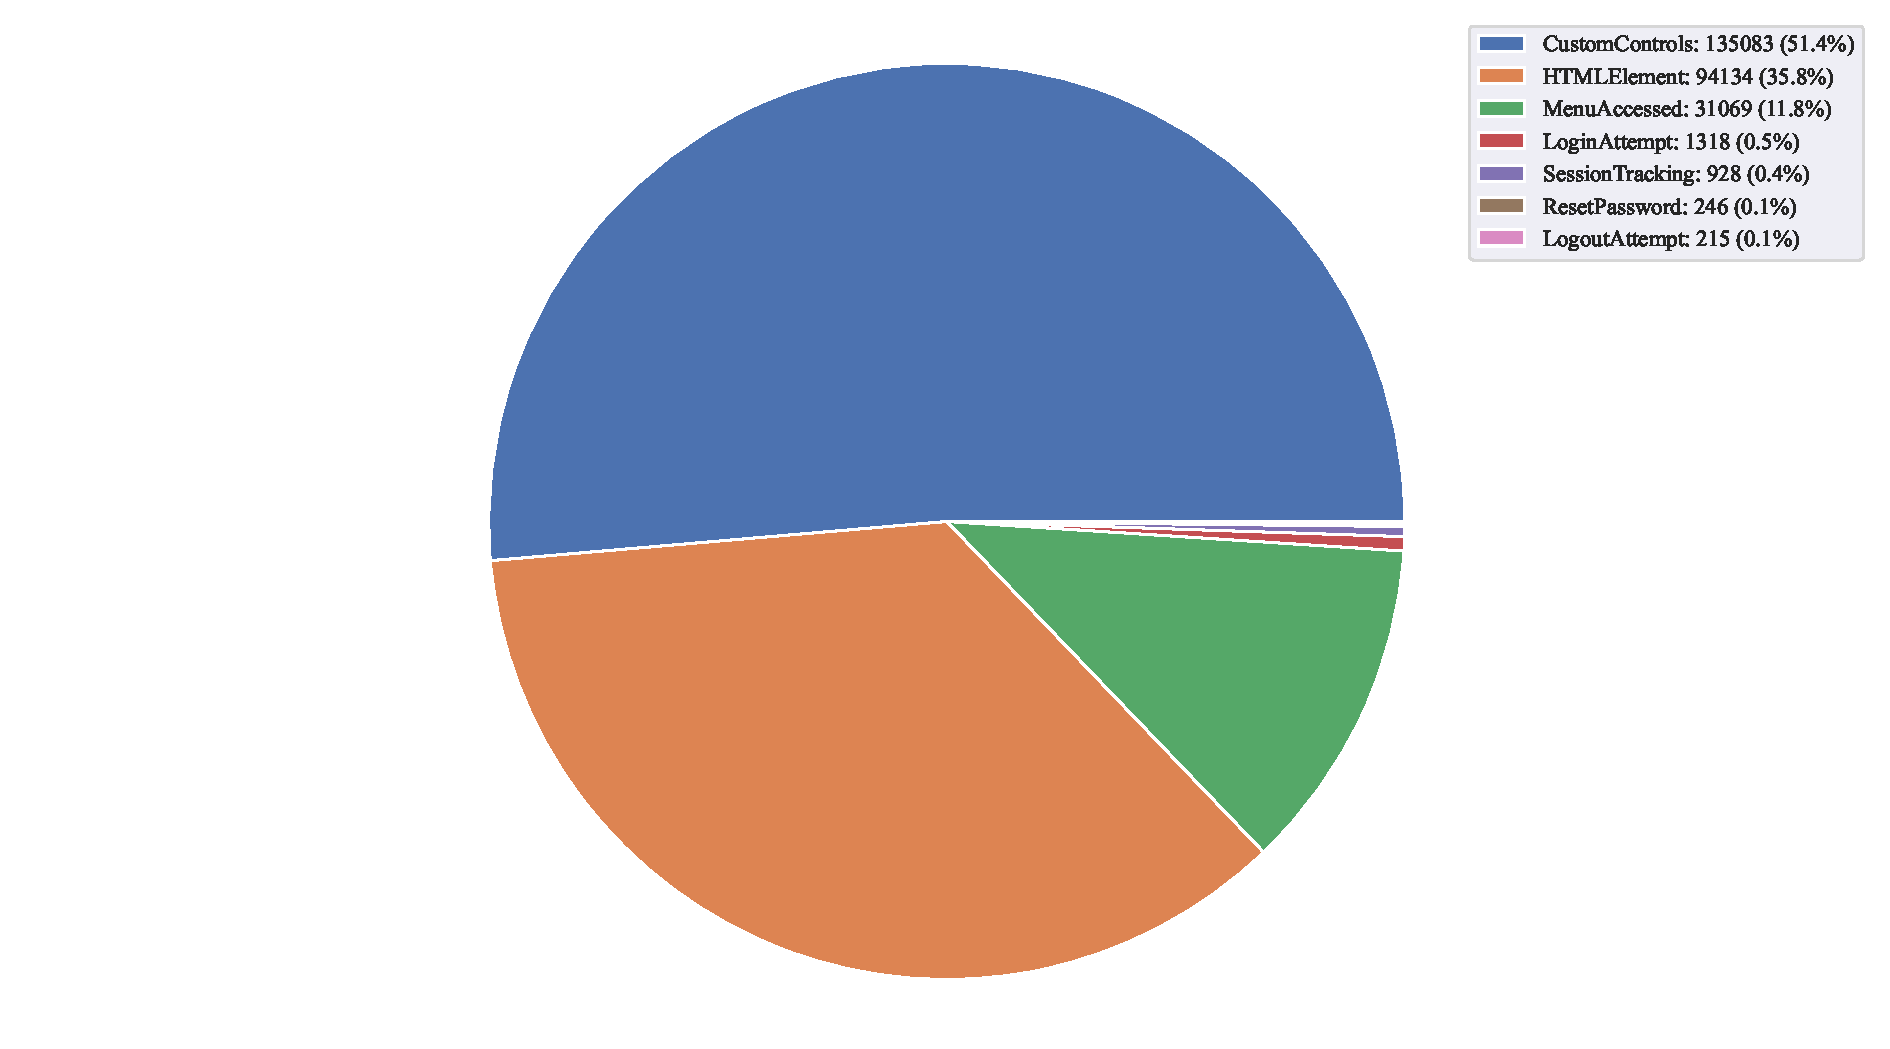
\includegraphics[width=0.95\linewidth]{img/ch3/analysis/case_C_breakdown.pdf}
	\caption[User activity types breakdown of Case Study C]
	{\textit{User activity types breakdown of Case Study C}}\label{fig:ch3_caseCBreakdown}
\end{figure}

According to the breakdown of user activities in \Cref{fig:ch3_caseCBreakdown}, most user activities for Case Study C is \texttt{CustomControl} user activity type. The more the user interacts with the system, the more the total amount of the general user activity types (\texttt{CustomControl} and \texttt{HTMLElement}) increases. \Cref{fig:ch3_caseCAnalysis} is a breakdown of the user activity of each subsystem's utilisation.

\clearpage

\begin{figure}[!htb]
	\centering % cent the figure
	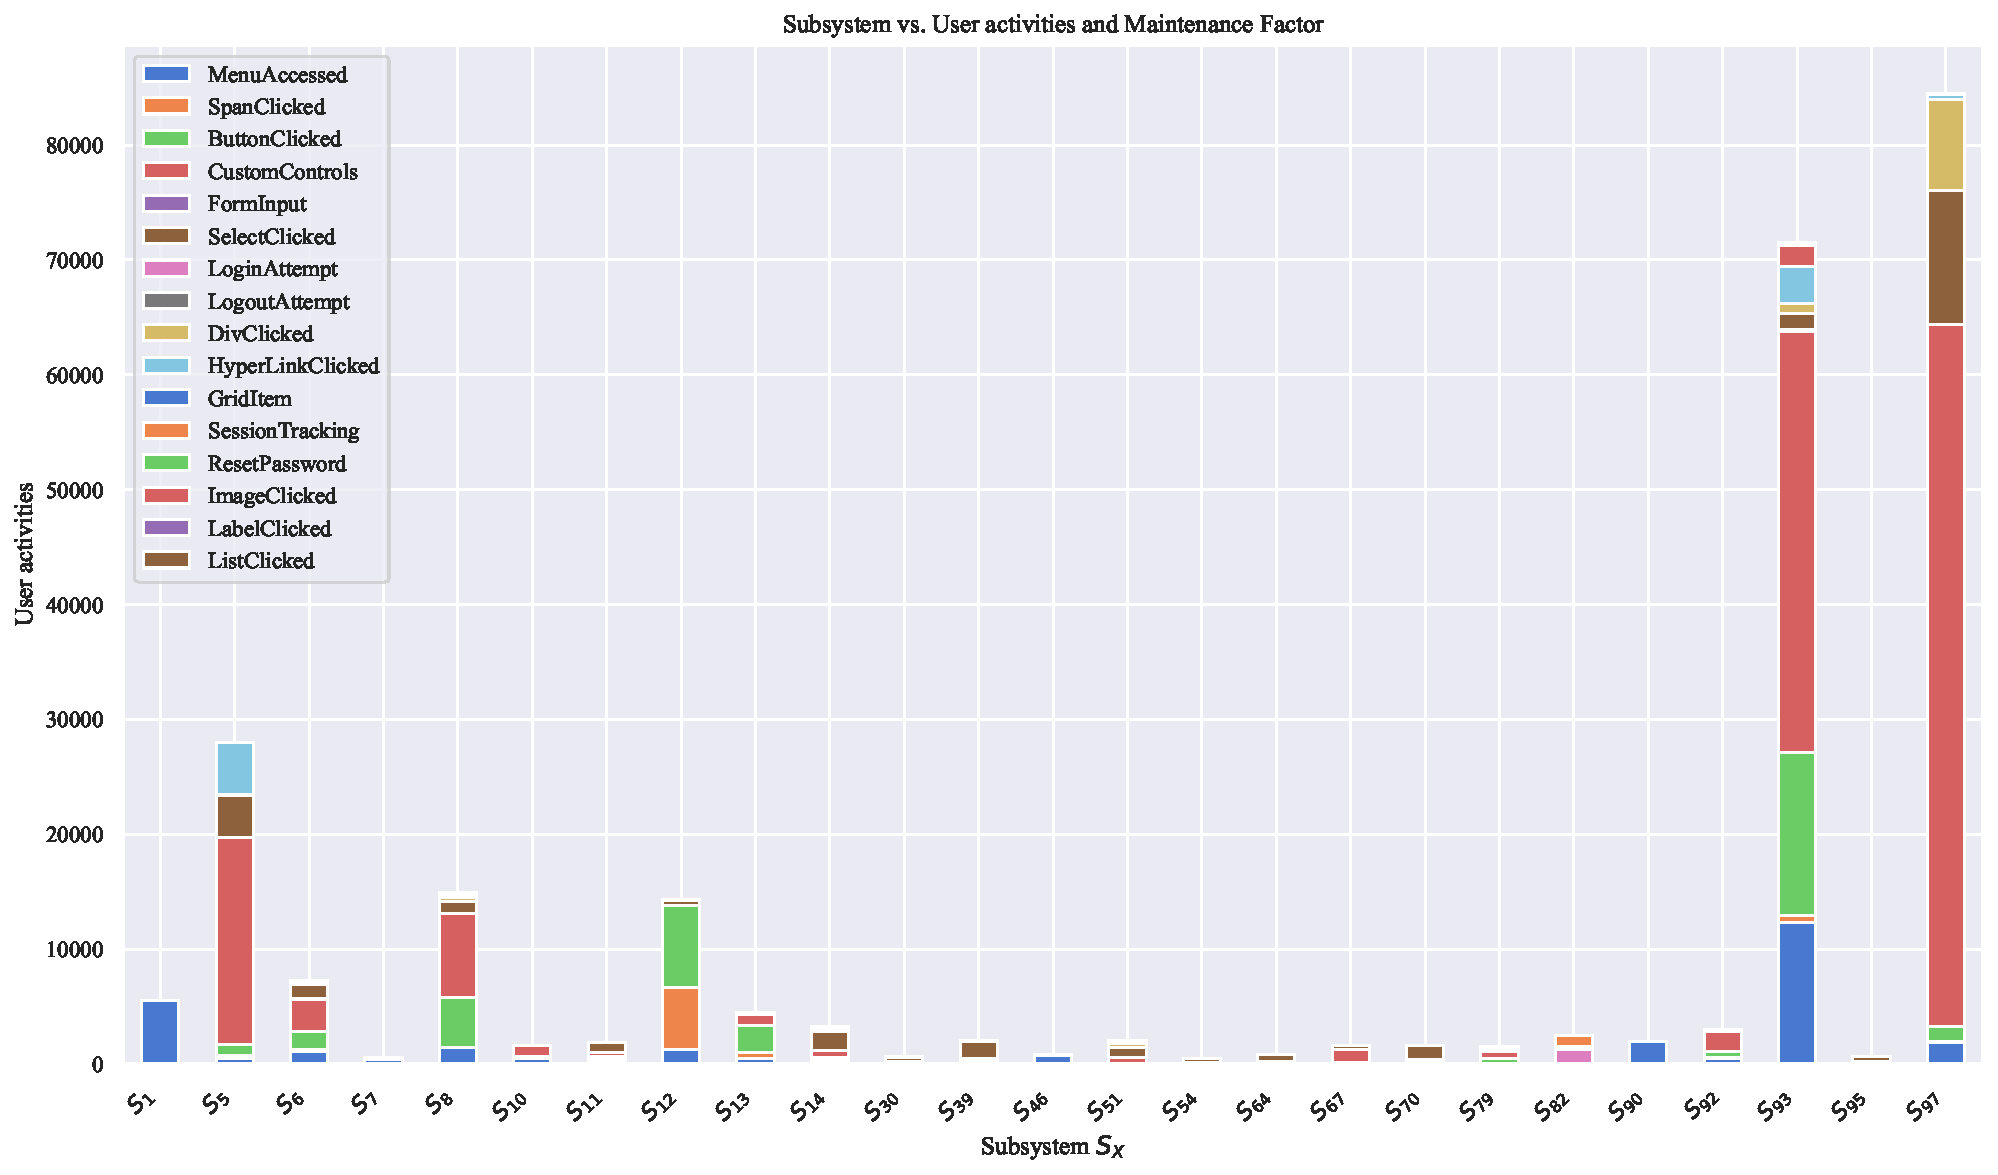
\includegraphics[width=0.95\linewidth]{img/ch3/analysis/case_C_subsystems_1.pdf}
	\caption[System utilisation breakdown of Case Study C]
	{\textit{System utilisation breakdown of Case Study C}}\label{fig:ch3_caseCAnalysis}
\end{figure} 

In \Cref{fig:ch3_caseCAnalysis} the total captured user-based event logs are dominated by $S_{97}$, $S_{93}$ and $S_{12}$. Most user-based events are general activity types for all the subsystems, as this case study is used for configuration purposes. Editing these configurations will create more general user activity types than other types of user activity. The log quality assessment for Case Study C is discussed in \Cref{tbl:ch3_caseCQuality}. \par \Cref{tbl:ch3_caseCQuality} indicated that logging attributes were missing for some types of user activity. This is not as severe as the incomplete logging attributes of Case Study B. It is expected that the main purpose of these activity types is to track log-in and log-out attempts.

\begin{xltabular}{\textwidth}{clcX}
	\caption[Logging quality assessment of Case Study C]{\textit{Logging quality assessment of Case Study C}}\label{tbl:ch3_caseCQuality}\\
	\toprule
	\thead{Req. ID} & \thead{Description} & \thead{Achieved} & \thead{Comments} \\
	\midrule
	\endfirsthead

	\caption[]{\continueCaption} \\
	\toprule
	\thead{Req. ID} & \thead{Description} & \thead{Achieved} & \thead{Comments} \\
	\midrule
	\endhead

	\midrule
	\multicolumn{4}{r}{\continueText} \\ 
	\endfoot
	\endlastfoot

	\rowcolor{lightgray}
	\ref{fr:ur1} & Log availability & \cmark & \RaggedRight The log availability for Case Study C is: \begin{itemize}
			\item \textit{Locally complete} due to most of the log attributes being available during the capturing phase of the event log. There are incomplete logs where log attributes were not obtained for user activity types, such as the \texttt{LoginAttempt}. The user's identity is not yet known on some of the captured event logs. As seen in Case Study A, this case study uses a central logging point for the client- and server-side.
			\item \textit{Globally complete} due to using a single log point on the client and server side of the main software system that captures events in most of the subsystems. 
		\end{itemize} \\
	\ref{fr:ur2} & Log completeness & \cmark & The logging attributes are complete for all the subsystems, as no other post-logging operations are needed to fix some of the logs. \\
	\rowcolor{lightgray}
	\ref{fr:ur3} & Log extraction & \cmark & Although the availability and completeness of the event logs are mostly achieved, the log extraction process is still possible. \\
	\bottomrule
\end{xltabular}

\subsubsection{Maintenance prioritisation}
The maintenance prioritisation factor for the user activities in the upper quartile of the subsystem for Case Study C is calculated in \Cref{tbl:apx_caseC}.


    \begin{xltabular}{\textwidth}{XPPPP}
        \caption[Case study C's upper quartile maintenance pefromance]
        {\textit{Case study C's upper quartile maintenance pefromance}}
        \label{tbl:apx_caseC} \\
        \toprule
         \thead{$S_{X}$} & \thead{$P_N$}  & \thead{$A_N$} & \thead{$M_{PF}$} & \thead{$P_{R}$} \\
        \midrule
        \endfirsthead

        \caption[]{\continueCaption} \\
        \toprule
        \thead{$S_{X}$} & \thead{$P_N$}  & \thead{$A_N$} & \thead{$M_{PF}$} & \thead{$P_{R}$} \\
        \midrule
        \endhead

        \midrule
        \multicolumn{5}{r}{\continueText} \\ 
        \endfoot
        \endlastfoot
    \rowcolor{lightgray} $S_{97}$ & 1.0000 & 1.0000 & 1.0000 & 1 \\ 
  $S_{93}$ & 0.9931 & 0.8464 & 0.8405 & 2 \\ 
 \rowcolor{lightgray} $S_{12}$ & 0.5903 & 0.1694 & 0.1000 & 3 \\ 
  $S_{8}$ & 0.5625 & 0.1763 & 0.0992 & 4 \\ 
 \rowcolor{lightgray} $S_{5}$ & 0.2917 & 0.3312 & 0.0966 & 5 \\ 
  $S_{6}$ & 0.7083 & 0.0859 & 0.0608 & 6 \\ 
 \rowcolor{lightgray} $S_{1}$ & 0.8681 & 0.0660 & 0.0573 & 7 \\ 
  $S_{82}$ & 0.8681 & 0.0291 & 0.0253 & 8 \\ 
 \rowcolor{lightgray} $S_{14}$ & 0.5208 & 0.0391 & 0.0204 & 9 \\ 
  $S_{90}$ & 0.7778 & 0.0231 & 0.0180 & 10 \\ 
 \rowcolor{lightgray} $S_{13}$ & 0.3264 & 0.0529 & 0.0173 & 11 \\ 
  $S_{92}$ & 0.1736 & 0.0359 & 0.0062 & 12 \\ 
 \rowcolor{lightgray} $S_{11}$ & 0.2500 & 0.0223 & 0.0056 & 13 \\ 
  $S_{10}$ & 0.2778 & 0.0188 & 0.0052 & 14 \\ 
 \rowcolor{lightgray} $S_{46}$ & 0.4167 & 0.0095 & 0.0039 & 15 \\ 
  $S_{67}$ & 0.1181 & 0.0194 & 0.0023 & 16 \\ 
 \rowcolor{lightgray} $S_{7}$ & 0.2778 & 0.0070 & 0.0019 & 17 \\ 
  $S_{70}$ & 0.0833 & 0.0197 & 0.0016 & 18 \\ 
 \rowcolor{lightgray} $S_{95}$ & 0.1597 & 0.0076 & 0.0012 & 19 \\ 
  $S_{39}$ & 0.0417 & 0.0238 & 0.0010 & 20 \\ 
 \rowcolor{lightgray} $S_{79}$ & 0.0347 & 0.0182 & 0.0006 & 21 \\ 
  $S_{64}$ & 0.0625 & 0.0100 & 0.0006 & 22 \\ 
 \rowcolor{lightgray} $S_{51}$ & 0.0208 & 0.0245 & 0.0005 & 23 \\ 
  $S_{54}$ & 0.0486 & 0.0056 & 0.0003 & 24 \\ 
 \rowcolor{lightgray} $S_{30}$ & 0.0278 & 0.0077 & 0.0002 & 25 \\
        \bottomrule
    \end{xltabular}
    

The upper quartile of the maintenance performance of the subsystems of \Cref{tbl:apx_projectC_Normilised} in \Cref{tbl:apx_projectC_Normilised} is used to create the results of \Cref{tbl:apx_projectC_Normilised} using \Cref{eq:ch2_eventNormalised,eq:ch2_maintenanceFactorSimplified,eq:ch2_priorityNormalised}. The results of \Cref{tbl:apx_caseC} are visually presented in \Cref{fig:ch3_caseCAnalysis}.\par The high usage of $S_{97}$, $S_{93}$, and $S_{12}$ with a high number of users linked to each one increased their maintenance priority factor. Other systems such as $S_{6}$, $S_{1}$ and $S_{82}$ have a higher priority normalisation than $S_{12}$, but they have a significantly lower normalisation of user activity.

\subsection{Critical analysis results}\label{sec:ch3_criticalAnalysis}

\subsubsection{Summary of comparison between case studies}
The three case studies discussed respectively \Cref{sec:ch3_csA,sec:ch3_csB,sec:ch3_csC} have similarities and differences. The logging mechanism used for Case Study A and Case Study C is similar, and both case studies make use of the MVC architecture discussed in \Cref{sec:ch2_webApplicationArchitecture}:

\begin{itemize}
	\item Both systems have a modified application of the \Cref{sec:ch3_ElementObtaining} client-side event log to obtain the HTML element with which the user interacts.
	\item Using action filters in \texttt{C\#} to create a single log point on the server side to capture user-based events. 
	\item The log quality of these two case studies is similar since both systems would identify user-based events through the action filter used as a logging point.
\end{itemize}

The older subsystems of Case Study C use multiple logging points in the logging mechanism to capture logs. The same user-based event types defined in \Cref{tbl:ch3_systemAActivityTypes} of Case Study A were also identified. Case Study C has, therefore:

\begin{itemize}
	\item More logging points than Case Studies A and B. 
	\item A higher chance in the variance of the log quality than Case Study A and B's logging points. Different subsystems require modification of the logging points to ensure that the user-based event logs are captured for Case Study C.
	\item Decreased adaptability and maintainability due to the increased logging points.
\end{itemize}

Each case study had different breakdowns of their types of user activity. For Case Study A and B, which have the same kind of user activity, the analysis of \Cref{fig:ch3_caseABreakdown,fig:ch3_caseBBreakdown} had different results respectively. Most of Case Study B's event types were \texttt{Dash} due to how the system works, refreshing the entire page to obtain new data. \par There weren't many \texttt{DetailView} activity types for these older subsystems with a more straightforward design as Case Study B's subsystem. Approximately $30\%$ of Case Study B's activities were \texttt{DetailView}. The more complex subsystems requiring more user input increased this user type's share of the total captured logs. \par These logs could have been categorised into other more descriptive user activity types, such as with Case Study C. This was not necessary for Case Study A because the purpose of its maintenance priority is more comparable to the software system in Case Study B, which has a similar operational goal. \par All three case studies' user-based event logs are stored in a structured database with Case Study A and B using the same data structures. Case Study A and Case Study B use the same analysis procedures for the log analysis. \par Case Study C's logs did not have a corresponding subsystem data table for log analysis. Additional post-logging operations group all the different request URLs into subsystems. For the more complex and more extensive software system used in Case Study C, it was preferable to use this method to categorise logs into subsystems using the request URLs target controller file. \par Priority normalisation for Case Study A was superior and had a higher impact on the maintenance priority factor than Case Study A and C. Even if there were systems with a higher total user activity, the total number of active users had a more significant impact than the number of activities for most subsystems. \par Case Study B's highest subsystem ranked for maintenance priority had all the highest normalised priority and user activities. This subsystem is a home page that all users can access and use to navigate the rest of the system. \par Case Study C had two subsystems with a maintenance priority factor greater than $0.1$. Even if many users have been active in a subsystem, the number of captured user activities impacted the maintenance priority factor more than in Case Studies A and B.

\subsubsection{Value added per case study}
In each case study, some obstacles must be overcome to create a suitable logging mechanism for log analysis. Some of the unique obstacles and the value added for each case study include:

\begin{itemize}
	\item \textbf{Case Study A}
		\begin{itemize}
			\item This case study provides insightful data for management on which systems can be used for more strategic business decisions and the services provided to the end user.
		\end{itemize}
	\item \textbf{Case Study B}
	\begin{itemize}
		\item This case study made use of multiple logging points. Each logging point had unique obstacles to overcome to ensure that log quality was consistent and appropriate for log analysis.
		\item There are multiple old subsystems for this case study. The lack of activity on some of these systems provides evidence that these systems are no longer used.
	\end{itemize}
	\item \textbf{Case Study C}
	\begin{itemize}
		\item The additional logging types for the user's session changes provided logs to monitor the user's access to the system.
		\item The capture of the request parameters stored in the metadata log attributes provides additional information for developers to troubleshoot errors or bugs in the software system. Developers don't need direct aid from the user to understand what sequence of actions they perform to receive a certain response from the system.
		\item Multiple subsystems provided the same functionality. The subsystems used more regularly are updated with any missing functionality from the less regularly used subsystems. This reduced the number of subsystems and possibly integrated similar functionality into one subsystem to improve the user experience. 
	\end{itemize}
\end{itemize}

\clearpage

\subsubsection{Summary of positive points}
From the observations made regarding each case study, some positive points can be summarised:

\begin{itemize}
	\item Similar architecture software systems can use the same logging points that do not require too many modifications.
	\item Log quality for similar logging mechanisms is approximately the same for software system comparison.
	\item Log analysis tools can be used on all captured logs when implementing the correct log extraction process.
	\item Log analysis can be used for maintenance priority factor calculations.
	\item The lowest ranked maintenance priorities can be reviewed if they still offer value to the software system.
\end{itemize}

\subsubsection{Summary of negative points}

\begin{itemize}
	\item Some systems needed additional logging points that were each modified to obtain the desired user-based event logs.
	\item Log quality may differ for different implementations of logging points. This can happen in the same software system with multiple logging points.
	\item Log quality may impact the maintenance priority factor since some variables can have extreme cases where values are notably high. Certain subsystems, such as a navigation page, do not have a meaningful impact on the user but are needed to use the rest of the system.
\end{itemize}

\clearpage

\subsubsection{Functional requirements addressed}
The functional requirements defined in \Cref{chap:2} for Case Studies A, B, and C are addressed in \Cref{tbl:ch3_functionalRequirements}.

\newcommand{\frHeader}{
	\toprule
	\thead{Req. ID} & \multicolumn{3}{c}{\thead{Case study}} \\ 
	\cmidrule(lr){2-4}
	& \thead{A} & \thead{B} & \thead{C} \\
	\midrule
}

    
\begin{xltabular}{\textwidth}{XYYY}
    \caption[Functional requirements addressed]{\textit{Functional requirements addressed}}\label{tbl:ch3_functionalRequirements} \\
    
    \frHeader
    \endfirsthead
    
    \caption[]{\continueCaption} \\
    \frHeader
    \endhead
    
    \midrule
    \multicolumn{4}{r}{\continueText} \\ 
    \endfoot
    \endlastfoot
    
    % Add your functional requirements and case study information here
    \multicolumn{4}{c}{\thead{Log attributes (\ref{fr:logAttributes})}} \\ 
    \midrule
    \rowcolor{lightgray}
    \ref{fr:requirementsUserBased1} & \cmark & \cmark & \cmark \\
    \ref{fr:requirementsUserBased2} & \cmark & \cmark & \cmark \\
    \rowcolor{lightgray}
    \ref{fr:requirementsUserBased3} & \cmark & \cmark & \cmark \\
    \ref{fr:requirementsUserBased4} & \cmark & \cmark & \cmark \\
    \rowcolor{lightgray}
    \ref{fr:requirementsUserBased5} & \cmark & \cmark & \cmark \\
    \ref{fr:requirementsUserBased6} & \cmark & \cmark & \cmark \\
    \rowcolor{lightgray}
    \ref{fr:uatType1} & \cmark & \cmark & \cmark \\
    \ref{fr:uatType2} & \xmark & \xmark & \cmark \\
    \rowcolor{lightgray}
    \ref{fr:uatType3} & \cmark & \cmark & \cmark \\
    \ref{fr:subLogAttributes} & \cmark & \cmark & \cmark \\
    
    % Logging point requirements
    \midrule
    \multicolumn{4}{c}{\thead{Logging point creation (\ref{fr:loggingPoints})}} \\ 
    \midrule
    \rowcolor{lightgray}
    \ref{fr:lp1} & \cmark & \cmark & \cmark \\
    \ref{fr:lp2} & \cmark & Mostly & \cmark \\
    \rowcolor{lightgray}
    \ref{fr:lp3} & \cmark & Mostly & \cmark \\
    \ref{fr:lp4} & \cmark & \cmark & \cmark \\
    \rowcolor{lightgray}
    \ref{fr:serverDatabase} & \cmark & \cmark & \cmark \\
    
    % Log analysis tool
    \midrule
    \multicolumn{4}{c}{\thead{Log analysis tools (\ref{fr:logAnalysis})}} \\ 
    \midrule
    \rowcolor{lightgray}
    \ref{fr:ur1} & \cmark & Mostly & \cmark \\   
    \ref{fr:ur2} & \cmark & Mostly & \cmark \\
    \rowcolor{lightgray}
    \ref{fr:ur3} & \cmark & \cmark & Mostly \\
    \ref{fr:ur4} & \cmark & \cmark & \cmark \\
    \rowcolor{lightgray}
    \ref{fr:ur5} & \cmark & \cmark & \cmark \\
    \ref{fr:ur6} & \cmark & \cmark & \cmark \\
    
    % Maintenance priority
    \midrule
    \multicolumn{4}{c}{\thead{Maintenance prioritising (\ref{fr:maintenancePrioritising})}} \\ 
    \midrule
    \rowcolor{lightgray}
    \ref{fr:utCategories1} & \cmark & \cmark & \cmark \\
    \ref{fr:utCategories2} & \cmark & \cmark & \cmark \\
    \rowcolor{lightgray}
    \ref{fr:utCategories3} & \cmark & \cmark & \cmark \\
    \ref{fr:mpr1} & \cmark & \cmark & \cmark \\
    \rowcolor{lightgray}
    \ref{fr:mpr2} & \cmark & \cmark & \cmark \\
    \ref{fr:mpr3} & \cmark & \cmark & \cmark \\
    \rowcolor{lightgray}
    \ref{fr:mpr4} & \cmark & \cmark & \cmark \\
    \bottomrule
\end{xltabular}

\Cref{tbl:ch3_functionalRequirements} indicates that the functional requirements for the logging attributes (\ref{fr:logAttributes}) defined in \Cref{tbl:ch2_loggingAttributesFunctionalRequirements} for all three case studies were met. In each case study, only user-based events were captured for the user activity types defined for each case study, and the log attributes captured from the user-based event were obtained. \par Case Study A and B did not meet the \ref{fr:uatType2} requirement. Session changes in user activity type were unnecessary for these case studies since internal and external users' actual interactions with the systems were more important, and no other session-related activities could contribute to the log analysis. \par The functional requirement of the logging point (\ref{fr:loggingPoints}) for Case Study A and C addressed all sub-functional requirements. Case Study B did not meet all requirements as \ref{fr:lp2} and \ref{fr:lp3} are not fully met. In this older system, using multiple logging points requires modifications for groups or individual subsystems. This can cause inconsistencies in log quality, as some potential user-based event logs may not be consistently identified. \par Log analysis functional requirements (\ref{fr:logAnalysis}) is done using and creating custom log analysis tools. Since user-based events could be efficiently obtained from the software system, the quality of the log (\ref{fr:logQuality}) for Case Study A and B was complete. \par Case Study B had lower log quality, as the availability and completeness of the logs were lower due to the use of multiple log points. The log extraction (\ref{fr:ur3}) for Case Study C was achieved mainly because additional post-logging activities with the log analysis tool had to be used to create subsystems using the logs.\par Through the log analysis, maintenance priority (\ref{fr:maintenancePrioritising}) could be performed for each case study. The results of each case study were evaluated by comparing the software maintenance prioritisation with the other case studies.

\subsubsection{Gaps identified}
By analysing the results of the case studies and the test, these gaps were identified for this study:

\begin{enumerate}
	\item Log quality is important for further analysis of user-based events. Improvement in the implementation of the logging mechanism can increase the following:
		\begin{itemize}
			\item Accuracy of the logging mechanism to capture logs,
			\item trustworthiness of more complete consistent logs, and
			\item decreased performance impact on the rest of the software system.
		\end{itemize}
	Applying more fundamentals of \Cref{fig:ch1_EventQModel} could have improved the logging mechanism. This should also improve the log quality, especially for implementing Case Study B's logging mechanism.
	\item The log analysis used \Cref{eq:ch2_priorityNormalised,eq:ch2_eventNormalised,eq:ch2_maintenanceFactorSimplified} to rank the maintenance priority of each subsystem. Each case study had outliers for one of the two main parameters used for \Cref{eq:ch2_maintenanceFactorSimplified}. Some gaps for this study with these parameters include:
		\begin{itemize}
			\item The normalised priority ($P_N$) uses the total active users. Some users were internal and external clients, and others were software developers. Adding weight to some of these user types can improve the impact that $P_N$ has on $M_{PF}$. Some users, such as developers, are significant users who can't determine whether a subsystem is important when external client users pay for the software system to use it.
			\item Normalised user activities ($A_N$) have a similar problem to $P_N$. There are less important user activity types, and adding weight to how important each user activity type is can improve log analysis. For Case Study C, some of the similar user activity types were grouped to form one user activity type. This can be used more, or user activity types should be better defined to be more distinct.
		\end{itemize}
\end{enumerate}

\section{Conclusion}
This chapter explored the implementation of the methodology defined in \Cref{chap:2} to create a logging mechanism for different case studies. A test system was used to initially verify the development of the solution before it was implemented in three different case studies. \par Log analysis was performed for all logs obtained for October 2022. The following was carried out for each case study:

\begin{itemize}
	\item Identification of the type of activity of the user,
	\item implementations of log-points,
	\item log analysis, comprising:
		\begin{itemize}
			\item user activity type breakdown
			\item priority normalisation
			\item normalisation of user activity
			\item maintenance priority factor calculation, and
		\end{itemize}
	\item maintenance priority ranking and recommendations. 
\end{itemize}

All results were compared for the case study. The overall result of the log analysis is that implementing a user-based event-logging mechanism can aid in prioritising software maintenance. Particular gaps that can improve maintenance prioritising were identified.
